%% LyX 2.0.0 created this file.  For more info, see http://www.lyx.org/.
%% Do not edit unless you really know what you are doing.
\documentclass[12pt,english]{article}
\usepackage[T1]{fontenc}
\usepackage[latin9]{inputenc}
\usepackage{subscript}
\usepackage{listings}
\usepackage{wrapfig}
\usepackage{graphicx}
\usepackage[usenames,dvipsnames,svgnames,table]{xcolor}

\makeatletter

%%%%%%%%%%%%%%%%%%%%%%%%%%%%%% LyX specific LaTeX commands.
%% Because html converters don't know tabularnewline
\providecommand{\tabularnewline}{\\}

\makeatother

\usepackage{babel}
\begin{document}

\title{\textbf{aML}\\
a-Mazing Language}


\author{Sriramkumar Balasubramanian (\textbf{sb3457})\\
 Evan Drewry (\textbf{ewd2106})\\
 Timothy Giel (\textbf{tkg2104})\\
 Nikhil Helferty (\textbf{nh2407})}

\maketitle
\pagebreak{}
\tableofcontents{}
\pagebreak{}

\section{Introduction}
A maze is a puzzle in the form of a series of branching passages through which a solver must a route. 
Actual mazes have existed since ancient times, serving as a means to confuse the traveler from finding
his or her way out. Since then, the idea behind mazes has been extrapolated to construct a set of 
puzzles designed to challenge people to solve or find the route.
 
While the concept of maze solving might seem too restricted, maze exploration in general can be 
extrapolated to other fields like Graph theory and topology. Apart from this, there exist more than one 
way to solve mazes, which has led to the rise of the time and space analysis of these approaches.  Also 
solving a maze can be likened to exploring a map which paves way for many practical uses of a language
for solving mazes.

Having justified the existence of a language to solve mazes, we now introduce AML (A-mazing Language) 
which can be used to solve mazes by feeding instructions to a bot which is located at the entrance to the maze at time 0.  The maze in question can either be defined by the user in the form of text files or can be randomly generated by the standard library functions. 
AML is designed to not only make the process of solving mazes easier to a programmer, but also to 
introduce programming to the common man through mazes. 

AML's design ensures the freedom of the user to implement many maze solving algorithms, while 
ensuring the ease of use of the language to traverse mazes. The language serves as an instruction set to 
the bot, hence the movement of the bot determines accessing of various data.  

\pagebreak
\section{Tutorial}
The syntax of aML is similar to a simplified version of Java, or C. The available instructions allow you to move a bot around a maze. You can define your own functions in order to program bots with complex behavior. aML will provide a simple Graphical User Interface of the bot navigating the maze (either randomly generated or provided in a .txt file).

aML has a limited set of data types for variables to take. The most basic types are integer, analogous to the Java int, and bool, like the Java boolean. A third, slightly more complex datatype is cell. This represents a cell in the maze. The programmer can't construct new cells as that would alter the maze, they can only set a cell variable equal to an existing cell of the maze in order to find out information about it. The fourth, and most complex datatype, is List<datatype> (such as List<integer>), which is a First In First Out List that behaves much like a linked list.

Users can define their own functions in aML. A function can either return a datatype (function x():integer) or be void and return nothing. Functions can be recursive (no looping constructs are offered). A special function is main, which must be void and parameterless. main is always the first function in any given program, and is the function that aML will call when the program is run.

\subsection{Making Your Own Maze}
If users wish to build a custom maze for the bot to navigate, then the maze text file must adhere to a certain format. The text file must be a sequence of integers delimited by whitespace. The first integer is the number of rows in the maze; the second, the number of columns. Then an integer follows for every cell in the maze: either a 0 for a "hole" (unwalkable), a 1 for a walkable cell, a 2 for the starting cell of the bot, and a 3 for a target cell for the bot (note it is possible to have multiple targets). The format can be clearly illustrated by the following example:
\\\\\\\\
\begin{center}
\begin{tabular}{c}
\begin{lstlisting}
5 6

0 1 1 1 0 0 
1 1 2 0 1 1
0 0 1 1 1 0
0 1 1 0 1 3
0 3 1 0 1 1         
\end{lstlisting}
\end{tabular}
\end{center}


\begin{figure}[htb]
\centering
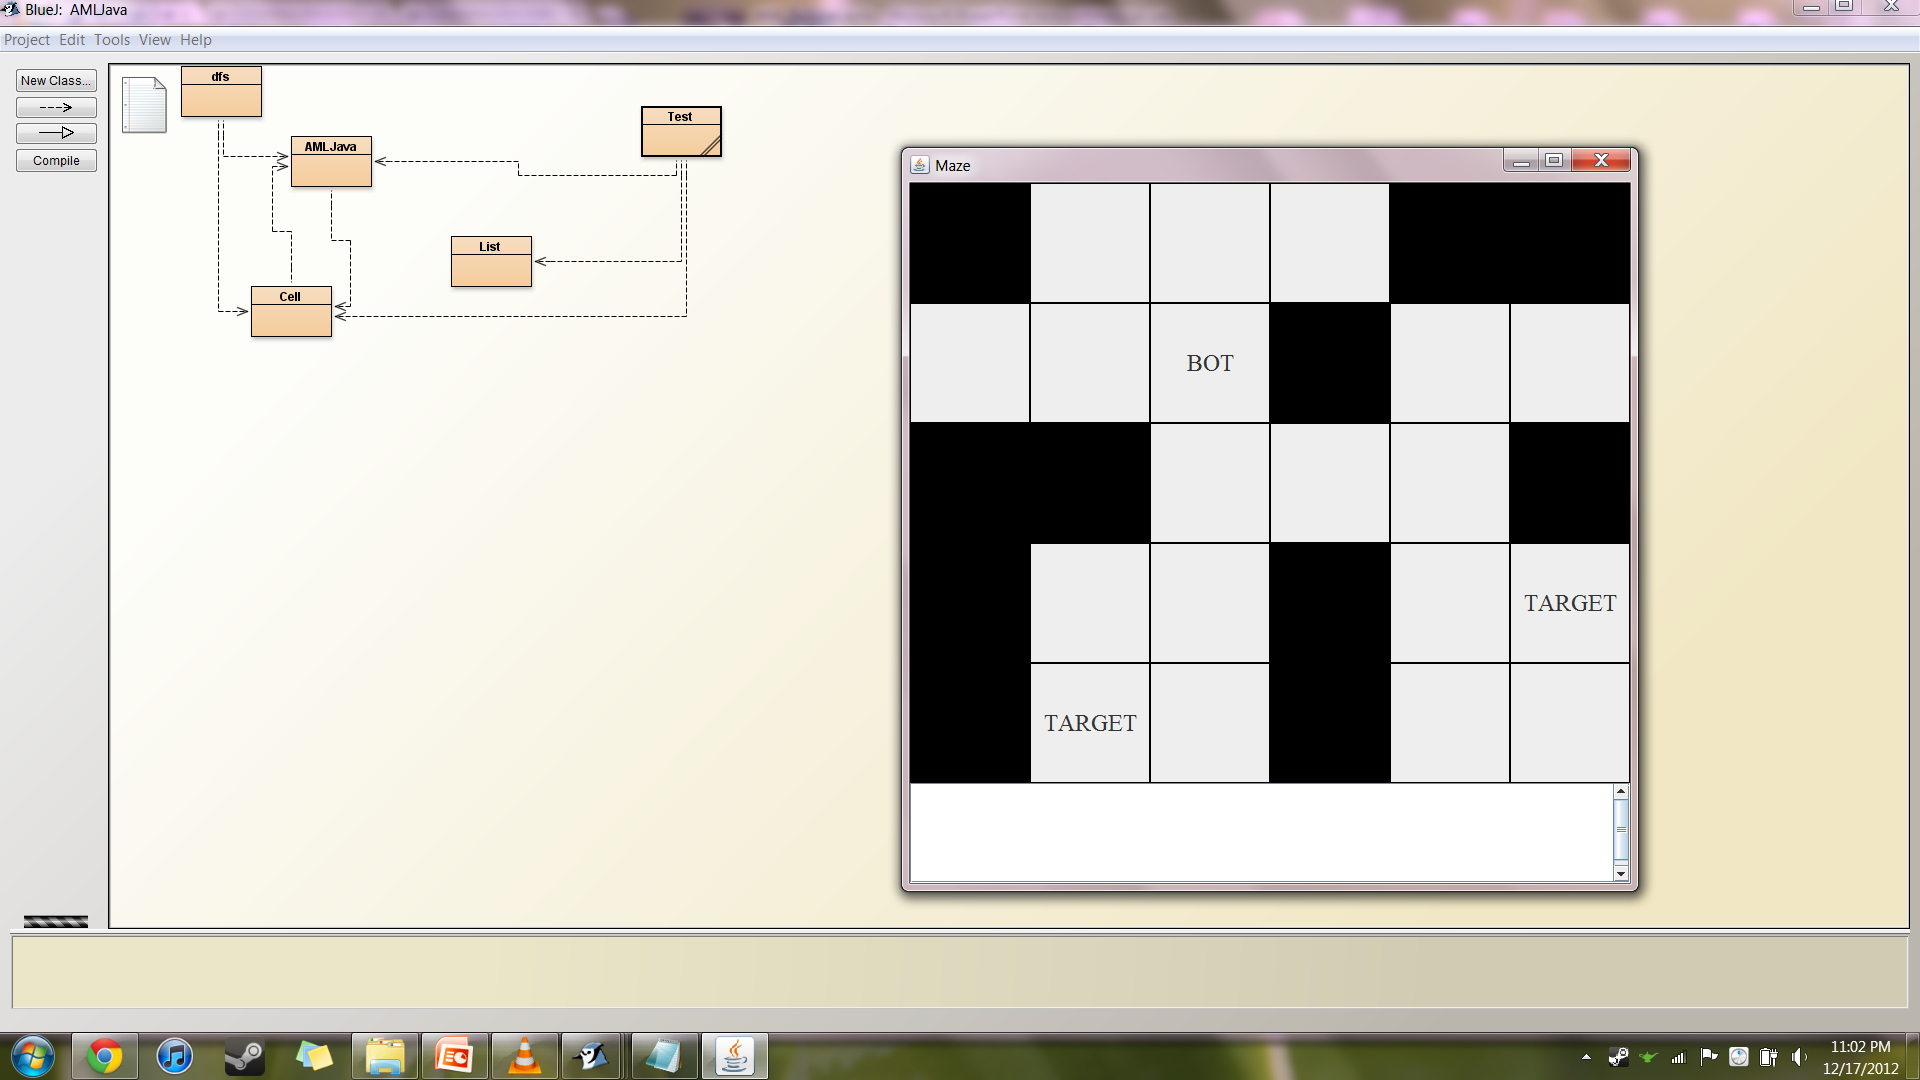
\includegraphics[height=80mm]{custommaze.png}
\caption{GUI representation of the text maze}
\end{figure}



\subsection{Example 1: Simple Program, Compilation}
Here is a very simple aML example:
\begin{center}
\begin{tabular}{c}
\begin{lstlisting}
#load-random

// function that is run by program initially
main():void {
	goRight();
}

function goRight():void {
	cell c := (CPos); // variables at start
	move_R(); // moves the bot to the right
	c := (CPos);
	if (NOT isTarget(c)) {
		goRight();
	}
} 
\end{lstlisting}
\end{tabular}
\end{center}

The first instruction in any aML program is the \#load instruction. This can either be \#load-random, which means aML will generate a random maze for you, or \#load<filename> which means you have a maze stored in filename.txt that you wish to be used. The main() function follows, and calls the recursive void function goRight(). goRight() instructs the bot to move right and check if the current cell (designated by the special variable CPos, standing for "current position") is the target. If not, it calls itself again. Obviously in most cases this bot will not be very effective and recurse endlessly (which amL will not stop from happening!), as in the case shown here:


\begin{figure}[htb]
\centering
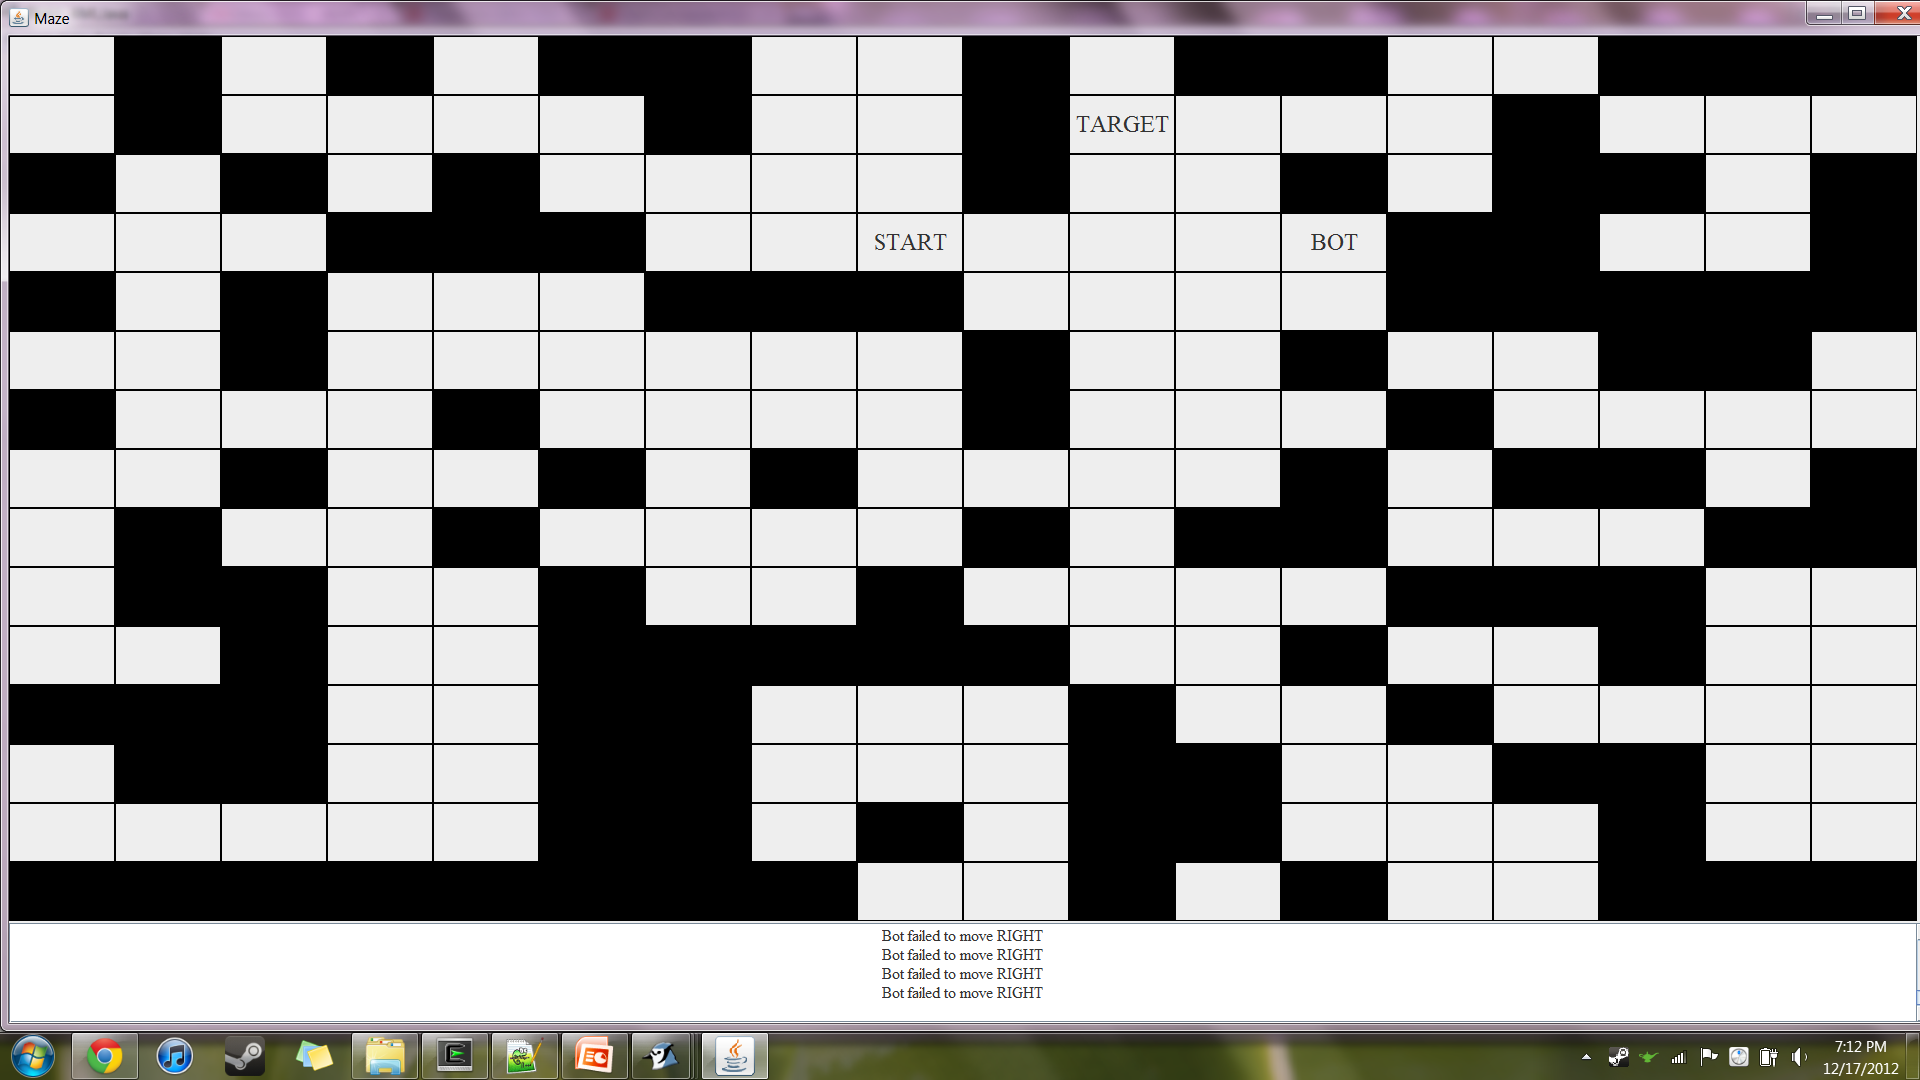
\includegraphics[height=80mm]{screenshot1.png}
\caption{GUI representation of the text maze}
\end{figure}


Another syntax rule in aML is that any variables in a function must be declared and initialized at the start of the function, prior to any other instructions. This is why cell c is initially set to a value before being reset after the use of the special move\_R() function (which instructs the bot to move right, if possible).

In order to compile an aML program, first construct aml.exe, which will compile the aML source code to an executable java program. In order to do this, use the provided makefile in the source files and simply type make into the command line. This will construct aml.exe. Then, if the example was in a file called example.aml, compile it by typing aml -c example.aml into the command line. This will construct a java program. Execute this by typing java example and the program will run.
	
	
\subsection{Example 2: Depth-First Search}
	It is possible to use aML to write much more complex functions than the first example. For example, here is a program that implements depth-first search:

\begin{lstlisting}
#load-random
main():void{
	DFS();
}



\end{lstlisting}


\begin{lstlisting}
function DFS():void{
	cell node := (CPos);
	
	if (isTarget(node)){
		exit();
	};
	
	if(myvisited(node)){
		DFS();
	};
	else{
		if (isSource(node)){
			exit();
		};

		revert();
		DFS();
	}
}



\end{lstlisting}


\begin{lstlisting}
function myvisited(cell node):bool{
	if (node.hasleft() AND NOT visited(node.left())){
		move_L();
	} else { if(node.hastop() AND NOT visited(node.up())){
		move_U();
	} else { if (node.hasright() AND NOT visited(node.right())) {
		move_R();
	} else { if(node.hasbottom() AND NOT visited(node.down())){
		move_D();
	} else {
		return false;
	}}}}
	return true;
}



\end{lstlisting}



Note the use of special functions such as node.hasright(), node.right(), revert() (which backtracks) and visited(cell c).

\subsection{Example 3: Greatest Common Denominator}
aML can also be used to implement a  simple mathematical function such as greatest common denominator, as in the following:


\begin{lstlisting}
#load-random

main():void{
	integer x := gcd(7,49);
	print(x);
	exit();
}

function gcd(integer n, integer m):integer{
	if(n = m){
		return n;
	};
	else{
		if (n > m) {
			return gcd(n - m, m);
		}
		else{
			return gcd(m - n,n);
		};
	};
}
\end{lstlisting}



\pagebreak{}
\section{Language Reference Manual}


\subsection{Introduction}

This manual describes the aML language which is used for manipulating
mazes and is used to provide instructions to a bot traversing the
maze. \\
The manual provides a reliable guide to using the language. While
it is not the definitive standard, it is meant to be a good interpretation
of how to use the language. This manual follows the general outline
of the reference manual referred to in \textquotedblleft{}The C Programming
Language\textquotedblright{}, but is organized slightly differently
with definitions specific to aML. The grammar in this manual is the
standard for this language.


\subsection{Lexical Conventions}

A program consists of a single translation unit stored as a file.
There are five classes of tokens: \textbf{identifiers}, \textbf{keywords},
\textbf{constants}, \textbf{operators}, and other separators. White
space (blanks, tabs, newlines, form feeds, etc.) and comments are
ignored except as they separate tokens. Some white space is required
to separate adjacent identifiers, keywords, and constants.


\subsubsection{Comments}

The characters // introduces a single line comment. The rest of the
line is commented in this case. This differs from a multi-line comment
which is enclosed by the /{*} and {*}/ characters. Multi-line comments
do not nest.


\subsubsection{Identifiers}

An identifier is a sequence of letters and digits, beginning with
a letter and can be of any length. The case of the letters is relevant
in this case. No other characters can form identifiers. \\
eg. abcd, Abcd, A123,abc1


\subsubsection{Keywords}

The following identifiers are reserved for use as keywords, and may
not be used otherwise:-\\
\\
\begin{tabular}{ccccccc}
if & return & display & remove & left & hasleft & integer\tabularnewline
then & main & print & add & right  & hasright & bool\tabularnewline
else & void & isSource & head & up  & hastop & list\tabularnewline
load & function & visited & next & down & hasbottom & cell\tabularnewline
random & exit & isTarget & isEmpty & CPos &  & \tabularnewline
true & null & NOT & AND &  &  & \tabularnewline
false &  &  & OR &  &  & \tabularnewline
\end{tabular}\\
\\
This language consists of many implicit variables and functions increasing
the size of the reserved words list. There are a few keywords like
display,null and next whose functionalities are not defined yet. But
they are reserved for future use.


\subsubsection{Literals}

There are different kinds of literals (or constants) in aML as listed
below:-


\paragraph{integer Literals}

An integer literal is taken to be decimal, and is of data type integer.
It may consist only of a sequence of digits 0-9. \\
eg. 0,1,22,-5


\paragraph{bool Literals}

A bool literal is either \textbf{True} or \textbf{False}, and is of
data type bool


\paragraph{list Literals}

The list literal can include either the integer, bool, cell or list<datatype>
types (cascaded lists). \\
eg. <{[}1{]}>,<{[}1,2,3{]}>,<{[}{[}1,2,3{]},{[}4,5{]}>,<{[}true, false,
true{]}>\\
.\\
As can be seen above the list literals consist of the form list<integer>,
list<list<....<list<integer>\textcompwordmark{}>...>\textcompwordmark{}>,
list<bool> or list<list ... <list <bool>\textcompwordmark{}> ... >\textcompwordmark{}>.
Details on list<datatype> and cell datatypes are provided in section
\ref{sec:Implicit-variables-and}. \\



\subsubsection{Separators}

The semi-colon \textbf{; }and the pair of braces \textbf{\{ \} },
the < > and {[} {]}, act as separators of the tokens. They are meant
to reduce ambiguity and conflicts during the parsing phase. The semi-colon
is added at the end of every statement to signify the end of the logical
statement. The \{ \} are used to collect groups of statements into
a single compound statement block. The < > and {[} {]} are used to
instantiate the list<datatype> variables.


\subsection{Syntax Notation}

In all of the syntactic notation used in this manual, the non-terminal
symbols are denoted in \textit{italics}, and literal words and characters
in \textbf{bold. }Alternative symbols are listed on separate lines.
An optional terminal or non-terminal symbol is indicated by subscripting
it with 'opt'. \\
eg. \textit{expression\textsubscript{opt}} denotes an optional expression


\subsection{Identifier interpretation}

aML interprets the identifier based on it's type. Each identifier
has a storage associated with it where a certain value is stored.
The type of the identifier determines the meaning of the values located
in the storage of the identifier. In aML each identifier's storage
exists as long as the block enclosing the identifier is being executed.\\
aML supports a 3 fundamental types:-\\

\begin{itemize}
\item integer - Objects declared as integers use 64 bits for storage and
are signed. They are primarily used for arithmetic operations.
\item bool - Objects declared as bools act as binary variables and can either
take the value \textbf{true} or \textbf{false}.
\item cell - A cell object stores the attributes of a cell of a maze.
\end{itemize}
There is one derived type list<type> which is used for storing lists
of objects of the fundamental types as well as the list type. By this
recursive definition, aML allows cascading of these lists.\\
 More details on the cell and list<type> datatypes is provided in
section \ref{sec:Types-revisited}.\\
\\
The complete data type definitions present in aML are as follows:-\\
\textit{}\\
\textit{datatype:-}\textbf{}\\
\textbf{\hspace*{0.5cm}integer}\\
\textbf{\hspace*{0.5cm}bool}\\
\textbf{\hspace*{0.5cm}cell}\\
\textbf{\hspace*{0.5cm}list<}\textit{datatype>}\\
\\
\textbf{Note:- }Each datatype is different from each other and no
two different datatypes can be combined together in a valid operation
defined in aML. Therefore there are no type-conversion rules defined
for aML.


\subsection{Expressions}

The complete syntax is provided in section \ref{sec:Syntax-summary}.
This section introduces the definition of the expression types which
are the basic building blocks of any language.


\subsubsection{Primary Expressions}

Primary expressions are identifiers, constants, or expressions in
parentheses. They also include the variable CPos which will be explained
in section \ref{sec:Types-revisited}.\\
\textbf{}\\
\textit{primary-expression:-}\\
\textit{\hspace*{0.5cm}identifier}\\
\textit{\hspace*{0.5cm}literal }\\
\textit{\hspace*{0.5cm}}( \textit{expression }\textbf{)}\textbf{\textit{}}\\
\textit{\hspace*{0.5cm}}\textbf{(CPos)}\\
 \\
An identifier is a primary expression provided it's type is specified
in it's declaration.\\
A literal is a primary expression. The type of the literal may include
integer, bool or list<type>. The syntax notation for literal including
the definition of list literals is given in detail in section \ref{sec:Syntax-summary}.
\\
A paranthesized expression is a primary expression whose type and
value are equal to those of the non-paranthesized one. \\
CPos refers to the current position of the bot in the maze. It is
a tracking variable and is used primarily to assign values to identifiers
of cell datatypes. \\
null is a constant which is assigned by default to identifiers of
the list<type> and cell datatypes. It signifies no storage allotted
to the identifier yet.


\subsubsection{Operators}


\paragraph{Arithmetic Operators}

There are six arithmetic operators:\{ +, -, {*}, /, \%, \textasciicircum{}\}.
The operands of these operators must be of integer data type. The
result will also be of type integer.\\
\textbf{}\\
\textit{arithmetic-expression:-}\\
\textit{\hspace*{0.5cm}expression + expression }\\
\textit{\hspace*{0.5cm}expression - expression }\\
\textit{\hspace*{0.5cm}expression {*} expression }\\
\textit{\hspace*{0.5cm}expression / expression }\\
\textit{\hspace*{0.5cm}expression \% expression }\\
\textit{\hspace*{0.5cm}expression \textasciicircum{} expression }\\
\\
\begin{tabular}{|c|c|c|}
\hline 
Operator & Semantic & Comments\tabularnewline
\hline 
\hline 
+ & addition & \tabularnewline
\hline 
- & subtraction & \tabularnewline
\hline 
{*} & multiplication & \tabularnewline
\hline 
/ & division & integer division only. Divide by zero => error\tabularnewline
\hline 
\% & modulo & \tabularnewline
\hline 
\textasciicircum{} & exponentiation & \tabularnewline
\hline 
\end{tabular}\\
\\



\paragraph{Relational Operators}

The relational operators all return values of bool type (either True
or False). There are six relational operators: \{==, \textasciitilde{}=,
>, <, >=, <=\}. The operators all yield \textbf{False} if the specified
relation is false and \textbf{True} if it is true. \\
\textbf{}\\
\textit{relational-expression:-}\\
\textit{\hspace*{0.5cm}expression}\textbf{\textit{ }}\textbf{== }\textit{expression}\\
\textit{\hspace*{0.5cm}expression}\textbf{ \textasciitilde{}= }\textit{expression}\\
\textit{\hspace*{0.5cm}expression}\textbf{ > }\textit{expression}\\
\textit{\hspace*{0.5cm}expression}\textbf{ < }\textit{expression}\\
\textit{\hspace*{0.5cm} expression}\textbf{ >= }\textit{expression}\\
\textit{\hspace*{0.5cm}expression}\textbf{ <= }\textit{expression}\\
\\
\begin{tabular}{|c|c|}
\hline 
Operator & Semantic\tabularnewline
\hline 
\hline 
== & equals\tabularnewline
\hline 
\textasciitilde{}= & not equals\tabularnewline
\hline 
> & greater\tabularnewline
\hline 
< & lesser\tabularnewline
\hline 
>= & greater than equals\tabularnewline
\hline 
<= & less than equals\tabularnewline
\hline 
\end{tabular}\\
\\
The \textbf{==} operator compares the value of left expression to
the right expression and evaluates to True if they are equal, False
otherwise. It is vice-versa for the \textbf{\textasciitilde{}= }operator.
The \textbf{> }operator evaluates to true if the left expression is
greater than the right expression, false otherwise. The \textbf{<
}operator behaves in the opposite manner. The \textbf{>= }and \textbf{<=
}operators check for equality condition as well. \\
For the == and \textbf{\textasciitilde{}= }operators, the expressions
involved must be of the same datatype. The other operators are defined
only for the integer datatype where comparison is meaningful. For
the cell datatype, the == and \textasciitilde{}= compare the cell
location in the map to which both the operands point to. As for the
list<type> datatype, the two operators check if two variables referencing
list datatypes point to the same list object.\\



\paragraph{bool Operators}

The bool operators all return values of bool type (either True or
False). There are three bool operators: logical-NOT, logical-AND and
logical-OR, denoted by NOT, AND, and OR, respectively. \\
\textbf{}\\
\textit{not-expression:-}\\
\textit{\hspace*{0.5cm}}\textbf{NOT}\textit{ expression}\\
\textit{and-expression:-}\\
\textit{\hspace*{0.5cm}expression }\textbf{AND}\textit{ expression}\\
\textit{or-expression:-}\\
\textit{\hspace*{0.5cm}expression }\textbf{OR}\textit{ expression}\\
\\
The operand(s) to NOT, AND and OR have to evaluate to True or False,
or in other words, they must either be bool variables or relational
expressions. NOT negates the operand, AND returns True if all operands
evaluate to true, False otherwise. OR returns True if at least one
of the operands evaluate to true, False otherwise.


\paragraph{Assignment Operators}

There is a single assignment operator in aML, \textbf{:=,} which does
simple assignment. It is a binary operator which assigns the value
of the right operand to the storage of the left operand.\\
\\
\textit{assignment-expression:-}\\
\textit{\hspace*{0.5cm}identifier }\textbf{:=}\textit{ expression}\\
\textit{}\\
The type of the expression must be identical to the type of 'lvalue'.


\paragraph{Associative Operator}

The \textbf{. }operator is used for function calls on variables represented
by identifiers. The structure of statements involving the operator
is shown in section\ref{sec:Syntax-summary}.


\subsection{Declarations}

Declarations specify the interpretation given to each identifier i.e.
the type of data it can point to and the associated operations that
go along with it. Declarations can be divided into variable and function
declarations. Variable declarations refers to the declaration of identifiers
whose type belongs to one of the datatypes mentioned and is different
from function declarations both syntactically and semantically.


\subsubsection{Variable Declarations\label{sub:Variable-Declarations}}

The rule representing the declaration of identifiers is listed in
the complete Syntax summary in section \ref{sec:Syntax-summary}.
The declaration of identifiers is similar to many strongly typed languages
where thet type associated with the identifier must be specified during
declaration. In aML variable declaration is allowed only at the beginning
of the main method and other functions. Without any loss of generality
variable declaration is not allowed to intermix with statements and
also it is encourage that while declaring variables at the top, they
are assigned to literal values initally, or function calls, but not
other variables. They can be assigned to subsequent variables using
assignment statements in the body of the function.\\
\\
\textit{declaration-expression:-}\\
\textit{\hspace*{0.5cm}datatype identifer := literal }\\
\textit{\hspace*{0.5cm}datatype identifier := }\textbf{(CPos)}\textit{
}\\
\textit{\hspace*{0.5cm}datatype identifier := lang\_functions}\\
\\
\\
Examples of some declarations are given below:-
\begin{itemize}
\item integer x;
\item bool flag;
\item cell node;
\item list<integer> mylist;
\end{itemize}

\subsubsection{Variable Initialization\label{sub:Variable-Initialization}}

When an identifier is declared, an initial value must also be specified.
The identifier can be re-initalized after it's declaration using assignment
statements. \\
 \textit{}\\
\textit{init-expression:-}\\
\textit{\hspace*{0.5cm}identifier} \textbf{:=} \textit{expression}\\
\\
Care must be taken to ensure that the identifer's type must be consistent
with the type of the expression.\\


A few examples of variable initializations are provided below;
\begin{itemize}
\item x := 10;
\item flag := false;
\item node := null;
\item mylist.head() := 1;
\end{itemize}
The exact rule is provided in the Syntax summary in section \ref{sec:Syntax-summary}.
Initialization can also be combined with declaration in a single step.
This is also shown in final section.


\subsubsection{Function Declaration}

Functions can either return a certain datatype or be void functions
(return no value). A function header is specified with the \textbf{function
}keyword and an identifier along with an optional argument list and
return type. Functions can be {}``used'' by function calls. But
for a function to be called, it must be declared in the program.\\
\\
\textit{function\_declaration:-}\\
\textit{\hspace*{0.5cm}function\_header}\textbf{ \{ }\textit{vdecl\_list
body}\textbf{ \}}\\
\textbf{}\\
\textit{function\_header:-}\\
\textit{\hspace*{0.5cm}}\textbf{function}\textit{ identifier (args\_list\textsubscript{\textbf{opt}})}\textbf{
: }\textit{return\_type}\\
\textit{}\\
\textit{args\_list:-}\\
\textit{\hspace*{0.5cm}datatype identifier}\\
\textit{\hspace*{0.5cm}datatype identifier}\textbf{,}\textit{ args\_list}\\
\textit{}\\
\textit{vdecl:}\\
\textit{\hspace*{0.5cm}datatype identifier := litera}\\
\textit{\hspace*{0.5cm}datatype identifier := }\textbf{(CPos)}\textit{
}\\
\textit{\hspace*{0.5cm}datatype identifier := lang\_functions}\\
\textit{}\\
\textit{vdecl\_list:}\\
\textit{\hspace*{0.5cm}empty declaration}\\
\textit{\hspace*{0.5cm}vdecl vdecl\_list}\\
\textit{}\\
\textit{body:-}\\
\textit{\hspace*{0.5cm}compound-statement}\textbf{}\\
\textbf{}\\
\textbf{}\\
Function calls are handled in section \ref{sec:Syntax-summary}. Compound
statements are described in detail in the section below. \\
Since function calls are part of compound statements, aML allows recursive
functions, which is necessary owing to the absence of any looping
constructs in this language. Also compound-statements do not allow
function definitions, so functions cannot be declared within functions.


\subsection{Statements}

Statements are usually executed in sequence, with the exception of
conditional statements. They are the next level of basic building
blocks after expressions. Each statement ends with a semi-colon at
the end which denotes the end of the logical statement. The physical
statement which is equivalent to one line in the editor may be comprised
of one or more logical statements.\\
One notable feature in aML is the lack of looping constructs. Iterations
are achieved by tail recursion of functions. The function definition
shown above is represented in the bigger picture in section \ref{sub:Program-Definition}.
The following definition gives an idea about the components of a statement.
The entire definition integrated with other definitions is present
in section \ref{sec:Syntax-summary}.


\subsubsection{Expression statement}

\textit{expression-statement:- }\\
\textit{\hspace*{0.5cm}expression}\textbf{;}\textit{ }\\
Expression statement consist of assignments and function calls. 


\subsubsection{Compound statements}

Compound statements are provided in the form:-\\
\\
 \textit{compound-statement:-}\\
\textit{\hspace*{0.5cm}}\textbf{\{ }\textit{statement-list }\textbf{\}}\textit{}\\
\textit{statement-list:-}\\
\textit{\hspace*{0.5cm}statement }\\
\textit{\hspace*{0.5cm}statement statement-list }\\
Compound statements are generally used to form the body of code to
execute in conditional statements, as well as the body of function
definitions.


\subsubsection{Conditional statements}

Conditional statements have the general form:-\\
\\
 \textit{conditional-statement:-}\textbf{}\\
\textbf{\hspace*{0.5cm}if }\textit{(expression)}\textbf{ then \{}\textit{compound-statement}\textbf{\};}\\
\textbf{\hspace*{0.5cm}if (}\textit{expression}\textbf{) then \{}\textit{compound-statement}\textbf{\}else
\{}\textit{compound statement}\textbf{\}}\\
\\
 The else branch is optional. The program will evaluate the expression
in parentheses, and if it evaluates to the bool value true then it
executes the corresponding compound-statement, and subsequently continues
on to the statement following the conditional statement. If the expression
does not evaluate to true, then the compound-statement following the
else branch is executed (if it exists). Branches are evaluated in
order, such that only the first branch with an expression that evaluates
to true will be executed, and all others skipped.


\subsubsection{Return statement}

Return statement Return statements take the form:-\\
\textit{return-statement:- }\\
\textit{\hspace*{0.5cm}}\textbf{return }\textit{expression}\textbf{;}\\
The expression should evaluate to a value of the return type of the
function being defined. 


\subsection{Scope rules}

Programs are not multi-file in AML, so external scope is not a worry.
The lexical scope of identifers is of relevance however. In brief,
subsequent to declaration a given identifier is valid for the rest
of the function inside which it was declared. Re-declarations using
an already declared identifier are not permitted. No identifiers can
be declared outside functions. \\
While user-defined variables cannot enjoy a global scope, the implicit
variables on the other-hand can do so. More information on implicit
variables is provided in \ref{sec:Implicit-variables-and}.


\subsection{Preprocessor directives}

Preprocessor directives must precede any code in the program. One
possible preprocessor directive takes the form: \textbf{\#load filename}.
This instruction ensures that the maze to be navigated is to be generated
from the file with name \textbf{filename}. (The file must be placed
in the 'maps' directory). The acceptable file format is pre-defined
and is independent of the language used. \\
Another possible directive is: \textbf{\#load-random}. This leads
to the maze is to be randomly generated each time the program runs.
\\
The two directives are mutually exclusive. In the event of multiple
directives, the compiler will show an error. 


\subsection{Implicit identifiers and functions\label{sec:Implicit-variables-and}}

aML consists of many implicit identifers or variables and functions.
By implicit, it follows that these identifiers can be used without
prior declaration as is the case for any user defined identifier or
function. However they cannot be modified by the user. Their usage
is mostly restricted to bool queries and assigning their values to
user-defined identifiers. The variables and functions along with their
meaing are provided below:-\\



\subsubsection{Variables}

The implicit variables are as follows.\\

\begin{itemize}
\item CPos - denotes the current position of the bot on the maze. Variables
of type cell can be instantiated by referencing CPos.
\item Visited - It is a dictionary like structure which maintains the 'visited'
status of each cell of the maze. It is used especially for backtracking
algorithms. It can never be used. The Visit() function provided accesses
this data structure inherently.
\end{itemize}

\subsubsection{Functions}

The implicit functions mainly deal with the movement and functionalities
of the bot. \\

\begin{itemize}
\item move\_U() - moves the bot one cell up from the current position, returns
true if it succeeds, false otherwise
\item move\_D() - moves the bot one cell down from the current position,
returns true if it succeeds, false otherwise
\item move\_L() - moves the bot one cell left of the current position, returns
true if it succeeds, false otherwise
\item move\_R() - moves the bot one cell right of the current position,
returns true if it succeeds, false otherwise
\item revert() - goes back to the previous position from the current position,
returns true if successful, false if at the start
\item visited(id) - checks if the cell refered to by id has been visited
or not
\end{itemize}

\subsection{Types revisited\label{sec:Types-revisited}}

This section discusses the list<datatype> datatype and the functions
associated with it. These two datatypes are in a sense less primitive
than the integer and bool datatypes. They come along with certain
functions which can be applied to variables belonging to these datatypes.
These functions are invoked or called using the \textbf{. }associative
operator on the identifier. The rule regarding the functions is shown
in the final section.


\subsubsection{list<datatype>}

The list<datatype> from it's definition in section\ref{sub:Variable-Declarations}
allows cascaded lists. This is especially useful for adjacency list
representation of graphs from mazes.\\
The functions associated with the datatype allow the manipulation
and traversal of the lists.\\

\begin{itemize}
\item add() - adds an elements to the end of the current list\\
eg. mylist.add(2);
\item remove() - removes and returns the first element of the current list\\
eg. mylist.remove();
\item isEmpty() - returns true if the current list has no elements, false
otherwise. \\
eg. mylist.isEmpty()
\item head() - returns the first element of the current list\\
eg. mylist.head();
\end{itemize}

\subsubsection{cell}

The cell datatype is unique in the sense that it cannot be set a user-defined
value. At any point of time, a variable of cell dataype can be assigned
only to the CPos value. It can however be stored in a variable which
will reflect that CPos value then, even if accessed at a later time.
\\
Certain functions are provided for this datatype which makes querying
the cell's content as well as it's neighborhood easier.


\paragraph{Neighborhood functions}
\begin{itemize}
\item left() - returns the left cell of the current cell if it exists and
the current cell has been visited
\item hasleft() - returns True if there is a cell to the left of the current
cell
\item right() - returns the right cell of the current cell if it exists
and the current cell has been visited
\item hasright() - returns True if there is a cell to the right of the current
cell
\item up() - returns the cell located upwards of the current cell if it
exists and the current cell has been visited
\item hasTop() - returns True if there is a cell to the top of the current
cell
\item down() - returns the cell located downwards of the current cell if
it exists and the current cell has been visited
\item hasbottom() - returns True if there is a cell to the bottom of the
current cell
\end{itemize}

\paragraph{cell functions}
\begin{itemize}
\item isTarget(id) - returns true if the cell is a target as specified in
the maze
\item isSource(id) - returns true if the cell is the start point of the
maze
\item get\_Loc(id) - returns the integer ID of the cell
\end{itemize}
Here id refers to an identifer pointing to a cell datatype.


\subsection{Syntax summary\label{sec:Syntax-summary}}

The entire syntax is provided below. This section is intended for
the logical understanding of the language structure rather than an
exact copy of the language.\\



\subsubsection{Expressions}

The expression includes declaration statements as well.\\
\\
\textit{expression:-}\\
\textit{\hspace*{0.5cm}primary\_expression}\\
\textit{\hspace*{0.5cm}lval\_expression}\textbf{}\\
\textbf{\hspace*{0.5cm}NOT }\textit{expression}\\
\textit{\hspace*{0.5cm}expression binop expression}\\
\textit{\hspace*{0.5cm}functions}\\
\textit{}\\
\textit{primary-expression:-}\\
\textit{\hspace*{0.5cm}identifier}\\
\textit{\hspace*{0.5cm}literal }\\
\textit{\hspace*{0.5cm}}( \textit{expression }\textbf{)}\textbf{\textit{}}\\
\textit{\hspace*{0.5cm}}\textbf{(CPos)}\\
\textbf{}\\
\textit{literal:-}\\
\textit{\hspace*{0.5cm}primitive\_literal}\\
\textit{\hspace*{0.5cm}}\textbf{<{[}}\textit{list\_literal\textsubscript{opt}}\textbf{{]}>}\textit{}\\
\textit{}\\
\textit{primitive\_literal:-}\\
\textit{\hspace*{0.5cm}integer\_literal}\\
\textit{\hspace*{0.5cm}bool\_literal}\\
\textit{}\\
\textit{list\_literal:-}\\
\textit{\hspace*{0.5cm}sub\_list}\\
\textit{\hspace*{0.5cm}}\textbf{{[}}\textit{list\_literal}\textbf{{]}}\textit{}\\
\textit{\hspace*{0.5cm}list\_literal,}\textbf{{[}}\textit{sub\_list}\textbf{{]}}\textit{}\\
\textit{}\\
\textit{sub\_list:-}\\
\textit{\hspace*{0.5cm}primitive\_literal}\\
\textit{\hspace*{0.5cm}primitive\_literal,sub\_list}\\
\textit{}\\
\textit{init-expression:-}\\
\textit{\hspace*{0.5cm}declarator := expression}\\
\textbf{}\\
\textit{datatype:-}\textbf{}\\
\textbf{\hspace*{0.5cm}integer}\\
\textbf{\hspace*{0.5cm}bool}\\
\textbf{\hspace*{0.5cm}cell}\\
\textbf{\hspace*{0.5cm}list<}\textit{datatype}\textbf{>}\\
\textbf{}\\
\textit{binop:-}\textbf{}\\


\begin{tabular}{|cccc|c|}
\hline 
 & Operators &  &  & Associativity\tabularnewline
\hline 
\hline 
\textasciicircum{} &  &  &  & Right\tabularnewline
\hline 
/ & {*} & \% &  & Left\tabularnewline
\hline 
> & < & >= & <= & Left\tabularnewline
\hline 
== & \textasciitilde{}= &  &  & Left\tabularnewline
\hline 
NOT &  &  &  & Right\tabularnewline
\hline 
AND &  &  &  & Left\tabularnewline
\hline 
OR &  &  &  & Left\tabularnewline
\hline 
:= &  &  &  & Right\tabularnewline
\hline 
\end{tabular}\\
\\
The binop table shows the binary operators in the decreasing order
of precedence (top - bottom) along with their associativity which
gives the fashion in which they are grouped together.\\
\\
\textit{functions:-}\\
\textit{\hspace*{0.5cm}list\_functions}\\
\textit{\hspace*{0.5cm}cell\_functions}\\
\textit{\hspace*{0.5cm}maze\_functions}\\
\textit{\hspace*{0.5cm}lang\_functions}\\
\textit{}\\
\textit{list\_functions:-}\textbf{}\\
\textbf{\hspace*{0.5cm}}\textit{identifier}\textbf{.remove()}\\
\textbf{\hspace*{0.5cm}}\textit{identifier}\textbf{.isEmpty()}\\
\textbf{\hspace*{0.5cm}}\textit{identifier}\textbf{.head()}\\
\textbf{}\\
\textit{cell\_functions:-}\textbf{}\\
\textbf{\hspace*{0.5cm}}\textit{identifier}\textbf{.left()}\\
\textbf{\hspace*{0.5cm}}\textit{identifier}\textbf{.right()}\\
\textbf{\hspace*{0.5cm}}\textit{identifier}\textbf{.up()}\\
\textbf{\hspace*{0.5cm}}\textit{identifier}\textbf{.down()}\\
\textbf{\hspace*{0.5cm}}\textit{identifier}\textbf{.hasleft()}\\
\textbf{\hspace*{0.5cm}}\textit{identifier}\textbf{.hasright()}\\
\textbf{\hspace*{0.5cm}}\textit{identifier}\textbf{.hastop()}\\
\textbf{\hspace*{0.5cm}}\textit{identifier}\textbf{.hasbottom()}\\
\textbf{\hspace*{0.5cm}isTarget(}\textit{identifier}\textbf{)}\\
\textbf{\hspace*{0.5cm}isSource(}\textit{identifier}\textbf{)}\\
\textbf{}\\
\textbf{}\\
\textit{maze\_functions:-}\\
\textit{\hspace*{0.5cm}}\textbf{visited}(\textit{identifier}\textbf{)}\\
\textbf{\hspace*{0.5cm}get\_Loc(}\textit{identifier}\textbf{)}\\
\textit{}\\
\textit{lang\_functions:-}\\
\textit{\hspace*{0.5cm}identifier}\textbf{(}\textit{actual\_args\textsubscript{\textbf{opt}}}\textbf{)}\\
\textbf{}\\
\textit{actual\_args:-}\\
\textit{\hspace*{0.5cm}primary\_expression}\\
\textit{\hspace*{0.5cm}primary\_expression}\textbf{, }\textit{actual\_args}\textbf{}\\
\textbf{}\\



\subsubsection{Statements}

Statements are logical sentences that can be formed by the language.
A compound statement is a group of statements occuring in a linear
fashion one after the other.\\
\textit{compound-statement}:\textbf{-}\\
\textbf{\hspace*{0.5cm}\{}\textit{statement-list}\textbf{\}}\\
\textbf{}\\
\textit{statement-list:-}\\
\textit{\hspace*{0.5cm}statement}\\
\textit{\hspace*{0.5cm}statement statement-list}\\
\textit{}\\
\textit{statement:-}\textbf{}\\
\textbf{\hspace*{0.5cm}}\textit{expression}\textbf{;}\\
\textbf{\hspace*{0.5cm}return }\textit{expression}\textbf{;}\\
\textbf{\hspace*{0.5cm}\{ }\textbf{\textit{statement-list}}\textbf{
\}}\\
\textbf{\hspace*{0.5cm}if (}\textit{expression}\textbf{) }\textit{statement}\textbf{;}\\
\textbf{\hspace*{0.5cm}if (}\textit{expression}\textbf{) }\textit{statement}\textbf{
else }\textit{statement}\textbf{}\\
\textbf{\hspace*{0.5cm}exit();}\\
\textbf{\hspace*{0.5cm}print(}\textit{expression}\textbf{);}\\
\textbf{\hspace*{0.5cm}}\textit{move\_functions}\textbf{;}\\
\textbf{\hspace*{0.5cm}}\textit{lang\_functions}\textbf{;}\\
\textbf{\hspace*{0.5cm}}\textit{identifier}\textbf{.add(}\textit{expression}\textbf{);}\\
\textit{}\\
\textit{}\\
\textit{move\_functions:-}\textbf{}\\
\textbf{\hspace*{0.5cm}move\_To(}\textit{identifier}\textbf{)}\\
\textbf{\hspace*{0.5cm}move\_U()}\textit{}\\
\textbf{\hspace*{0.5cm}move\_D()}\textit{}\\
\textbf{\hspace*{0.5cm}move\_L()}\textit{}\\
\textbf{\hspace*{0.5cm}move\_R()}\textit{}\\
\textbf{\hspace*{0.5cm}revert()}\textit{}\\
\textbf{}\\
\\
If the expression to 'if' does not evaluate to True or False, an error
will be thrown. 


\subsubsection{Program Definition\label{sub:Program-Definition}}

This subsection describes the structure of the program and functions
which are the biggest building blocks in aML. Every aML must have
one and only one main function through which the control passes to
the program. It must also have exactly one pre-processor directive
to load the maze. It can have an arbitrary number of functions though.
The program structure is defined below:-\\
\\
\textit{program:-}\\
\textit{\hspace*{0.5cm}empty\_program}\\
\textit{\hspace*{0.5cm}pre-process program}\\
\textit{\hspace*{0.5cm}func-def program}\\
\textit{}\\
\textit{\hspace*{0.5cm}}\\
\textit{pre-process:-}\textbf{}\\
\textbf{\hspace*{0.5cm}\#load-}\textit{identifier}\textbf{}\\
\textbf{\hspace*{0.5cm}\#load-random}\\
\textbf{}\\
func-def:-\textbf{}\\
\textbf{\hspace*{0.5cm}main():void \{}\textit{vdecl\_list statement-list}\textbf{\}}\\
\textbf{\hspace*{0.5cm}function}\textit{ identifier}\textbf{(}\textit{formal-args\textsubscript{\textbf{opt}}}\textbf{):}\textit{return-type}\textbf{\{}\textit{vdecl\_list
statement-list}\textbf{\}}\\
\textbf{}\\
\textit{formal-args\textsubscript{\textbf{opt}}:-}\\
\textit{\hspace*{0.5cm}datatype identifier}\\
\textit{\hspace*{0.5cm}datatype identifier}\textbf{,}\textit{formal-args}\textbf{\textit{}}\\
\textbf{\textit{}}\\
\textit{return-type:-}\\
\textit{\hspace*{0.5cm}datatype}\textbf{}\\
\textbf{\hspace*{0.5cm}void}\\
\textbf{}\\
\textit{}\\
\textit{vdecl:}\\
\textit{\hspace*{0.5cm}datatype identifier := literal}\\
\textit{\hspace*{0.5cm}datatype identifier := }\textbf{(CPos)}\textit{
}\\
\textit{\hspace*{0.5cm}datatype identifier := lang\_functions}\\
\textit{}\\
\textit{vdecl\_list:}\\
\textit{\hspace*{0.5cm}empty declaration}\\
\textit{\hspace*{0.5cm}vdecl vdecl\_list}\\
\textit{}\\

\pagebreak

\section{Architecture Design}
aML was designed in such a fashion that the aML syntax was similar to the java syntax making the translation to java much easier. Hence java was chosen to be the language to be  translated to. The standard library functions were provided in java, where the maze was visualized using the java Swing GUI.


Keeping this in mind, the architecture of aML was designed as shown below tracing the steps from character streams typed by the user all the way to compiled java bytecode.

\begin{figure}[htb]
\centering
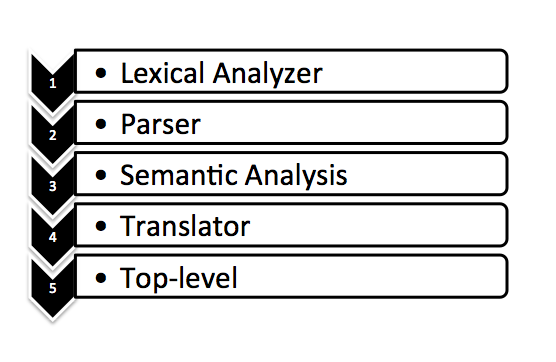
\includegraphics[height=80mm]{diagram.png}
\caption{Block diagram of the aML translator}
\end{figure}

\begin{enumerate}
\item
The lexical analyzer accepts a character stream and converts into a token stream. These tokens are defined in scanner.mll - the set of acceptable words in our language.  The token stream is passed onto the Parser.
\item
The Parser ensures that the token stream input received is consistent with the grammar rules defined in parser.mly -- the order in which the tokens can combine with each other forming the syntax of the language.  The parser while checking for grammar rule consistency forms the Abstract Syntax Tree or AST, with the help of the ast structures defined in ast.ml. This incidentally also contains the one-one mapping of ast nodes to translated java code.  The ast structure is passed onto the Semantic Analyzer.
\item
The Semantic Analyzer ensures that the syntax is actually meaningful. It ensures that the program defined by the user while conforming to the grammar actually make sense. For example the assignment of variables to values, the semantic analyzer ensures that the types have to be consistent for this to be a valid operation. The semantic analysis for aML is present in sast.ml.
\item
Once the semantic analysis is done and successful without throwing any exceptions, the verified ast structure can be translated to a .java file and compiled to .class (java bytecode). This is done in the file compile.ml. 
\item
The file toplevel.ml is provided for the user's convenience to run the program using the command line interface. The exact usage is shown on typing ./aml in the command line.
\end{enumerate}


\pagebreak

\section{Test Plan}

For our test suite, we decided to include both unit and functional tests for maximum coverage of our language's features. Both are necessary because alone, these two types of testing give only a limited guarantee of correctness, but together they ensure that everything works how it is supposed to. Unit tests test individual features in isolation, for example the correct translation of the addition operator or a function declaration. These are important because before we can even hope to ensure that our full codebase works properly, we must ensure that each unitary component provides the correct output for a given input. Because we didn't want to accidentally omit a feature of our language from the unit tests, our strategy for writing unit tests was to go through the LRM and create a test case for each feature described therein.  

Functional tests are at the other end of the testing spectrum -- they validate not a simple input-to-output conversion, but rather the result of complex interactions between many parts of the code. An example functional test case could be something like a GCD algorithm or a simple search algorithm. The reason we need functional tests on top of unit tests is that there is no way to verify that the pieces of our code work properly \textit{together }if we use only unit testing, which verifies that the pieces of our code work properly \textit{apart}. 

We decided to implement and automate our tests using bash script. All of this can be found in the tests subdirectory. Each individual test case has two components: (1) an aML source file containing the aML code relevant to the test case, and (2) a bash script file of the same name (but with a .test extension rather than a .aml extension) that contains the expected output from the test case as well as any other necessary information pertaining to the test case in question (for example, setting COMPILE\_ONLY=true if the test case is meant to cause an error on compilation). The bash file "test-base" contains all the functions necessary for automating the testing process, including functions to compile and run an individual test case, to print error/info data to the console, and to run the full suite at one time.


\pagebreak


\section{Lessons Learned}
\begin{itemize}
\item
One of the things that we learned is that a group should always start
early so that there is time to work out issues before deadlines. By
starting a little earlier on some sections, we may have been able to
avoid having to rush to fix certain issues before parts of the project
were due.
\item
Another thing we learned is the need to be flexible with your ideas
and not plan for a lot of features too early. A good approach would
have been to start simple and build off of simple features as we move
along. Planning for too many features caused us to have to change our
thinking at certain points during the project.
\end{itemize}



\subsection{Sriramkumar Balasubramanian}
\begin{itemize}
\item
Keep in frequent communication.
\item
Start earlier than you will.
\item
Spread the work out.
\item
Sleepless coding is inefficient and/or error-prone.

\end{itemize}
\subsection{Evan Drewry}
\begin{itemize}
\item
Being super organized is a very important factor in coding project as a team, especially when the team isn't always working together in the same room. Lack of organization can lead to confusion or wasted time for other group members who are also working on the project.
\item
Testing incorrect programs is as important as testing correct ones. If we only included meaningful and well-formed programs in our test suite, we would have no guarantee that our compiler responds appropriately to malformed input. Instead, we would only know that it respond appropriately to correct input.
\end{itemize}


\subsection{Tim Giel}
\begin{itemize}
\item
I learned that it is incredibly difficult to find a suitable time for everyone in a group to meet, especially 
when there are more people.  With everyone's schedule constantly changing and workloads piling up as the semester went on, it became increasingly difficult to find a time for everyone.  Fortunately, we were all pretty flexible and were able to meet as a group a lot which definitely helped in getting to know one another and how each of us work, which helped us work on our project more efficiently.
\item
I also learned that it is very tough when you don't have as much programming experience as others.  While we all were essentially learning two new languages (aML and OCaml), my lack of experience made me have to work a little harder than the other group members I think.
\end{itemize}



\subsection{Nikhil Helferty}
\begin{itemize}
\item
Keep in frequent communication.
\item
Start earlier than you will.
\item
Spread the work out.
\item
Sleepless coding is inefficient and/or error-prone.

\end{itemize}


\pagebreak{}

\section{Appendix}
\subsection{Lexical Analyzer}
\lstset{
language=[Objective]Caml,
basicstyle=\color{MidnightBlue}\footnotesize\ttfamily, % print whole listing small
columns=fullflexible,
keywordstyle=\color{violet}\bfseries,
% underlined bold black keywords
identifierstyle=\color{black}, % nothing happens
commentstyle=\color{gray}, % white comments
numbers=left, numberstyle=\tiny\color{gray}, stepnumber=1, numbersep=5pt
}
\begin{lstlisting}[caption=scanner.mll]
{open Parser}

let letter = ['a'-'z' 'A'-'Z']
let digit = ['0'-'9']

rule token = 
  parse [' ' '\t' '\r' '\n'] { token lexbuf }
| '+' { PLUS }
| '-' { MINUS}
| '*' { TIMES }
| '/' { DIVIDE }
| '%' { MOD }
| '^' { EXP }
| '.' { ASSOC }
| '(' { LPAREN }
| ')' { RPAREN }
| '{' { LBRACE }
| '}' { RBRACE }
| '[' { LSQUARE }
| ']' { RSQUARE }
| '<' { LSR }
| '>' { GTR }
| ';' { STMTEND }
| ',' { COMMA }
| ':' { RTYPE }
| '#' { HASH }
| ">=" { GTREQL }
| "<=" { LSREQL }
| "~=" { NEQ }
| "=" { EQ }
| ":=" { ASSIGN }
| "true" { TRUE }
| "false" { FALSE }
| "null" { NULL }
| "NOT" { NOT }
| "AND" { AND }
| "OR" { OR }
| "load" { LOAD }
| "random" { RANDOM }
| "return" { RETURN }
| "exit" { EXIT }
| "function" { FUNC }
| "main" { ENTRY }
| "void" { VOID }
| "print" { PRINT }
| "integer" { INTEGER }
| "bool" { BOOLEAN }
| "list" { LIST }
| "cell" { CELL }
| "if" { IF }
| "else" { ELSE }
| "display" { DISPLAY }
| "move_U" { MOVEUP }
| "move_D" { MOVEDOWN }
| "move_L" { MOVELEFT }
| "move_R" { MOVERIGHT }
| "move_To" { MOVETO }
| "get_Loc" { LOC }
| "isTarget" { ISTARGET }
| "visited" { VISIT }
| "isSource" { SOURCE }
| "revert" { REVERT }
| "left" { LEFT }
| "right" { RIGHT }
| "up" { UP }
| "down" { DOWN }
| "hasleft" { HASLEFT }
| "hasright" { HASRIGHT }
| "hastop" { HASTOP }
| "hasbottom" { HASBTM }
| "CPos" { CUR_POS }
| "add" { LISTADD }
| "remove" { LISTREMOVE } 
| "clear" { LISTCLEAR }
| "head" { LISTHEAD }
| "isEmpty" { LISTEMPTY } 
| ['-']?['1'-'9']digit*|'0' as amlex { NUM_LITERAL(int_of_string amlex) }
| letter(letter|digit)* as amlex { ID(amlex) }
| "/*" { multicmnt lexbuf}
| "//" { singlecmnt lexbuf}
| eof { EOF }

and multicmnt = 
	parse "*/" { token lexbuf}
|_ { multicmnt lexbuf}

and singlecmnt =
	parse "\n" { token lexbuf}
|_ { singlecmnt lexbuf}
\end{lstlisting}


\pagebreak


\subsection{Parser}

\begin{lstlisting}[caption=parser.mly]
%{ open Ast 
	let parse_error pErr = 
	print_endline pErr;
	flush stdout
%}

%token LPAREN RPAREN LBRACE RBRACE LSQUARE RSQUARE
%token PLUS MINUS TIMES DIVIDE MOD EXP 
%token ASSOC ASSIGN
%token GTR LSR GTREQL LSREQL NEQ EQ 
%token TRUE FALSE
%token STMTEND COMMA RTYPE HASH 
%token EXIT RETURN FUNC ENTRY VOID LOAD RANDOM NULL
%token INTEGER BOOLEAN CELL LIST
%token IF ELSE PRINT DISPLAY 
%token MOVEUP MOVEDOWN MOVELEFT MOVERIGHT MOVETO CUR_POS
%token ISTARGET VISIT SOURCE REVERT LOC
%token LEFT RIGHT UP DOWN HASLEFT HASRIGHT HASTOP HASBTM 
%token LISTADD LISTREMOVE LISTCLEAR LISTHEAD LISTEMPTY
%token AND OR NOT
%token <string> ID
%token <int> NUM_LITERAL
%token EOF

%nonassoc ELSE
%left GTR LSR GTREQL LSREQL NEQ EQ 
%left PLUS MINUS
%left TIMES DIVIDE
%left MOD
%right ASSIGN EXP
%left OR
%left AND
%right NOT

%start program
%type <Ast.program> program 

%%

program: 
  /* empty code */	{ [] }
| program pre_process { $2 :: $1 }
| program func_decl { $2 :: $1 }

pre_process:
	HASH LOAD LSR ID GTR  { Load($4) }
| HASH LOAD MINUS RANDOM { Load("random") }

func_decl:
	ENTRY LPAREN RPAREN RTYPE VOID LBRACE vdecl_list stmt_list RBRACE 
		{ Main({
			mainId = "main";
			mainVars = List.rev $7;
			body = $8;
			})
		}  
|	FUNC ID LPAREN formal_args RPAREN RTYPE return_type 
    LBRACE vdecl_list stmt_list RBRACE		
		{ Func({
			funcId = $2;
			formalArgs = List.rev $4;
			reType = $7;
			localVars = List.rev $9;
			statements = $10;
		})
		}
	
return_type:
   VOID { Void }
|  data_type { Data($1) }

data_type:
	INTEGER	{ Integer }
	|CELL     { Cell } 
	|BOOLEAN  { Bool }
	|formal_list { $1 }

formal_list: 
	|LIST LSR data_type GTR { List($3) }
			
formal_args: 
	/* no arguments */ { [] }
	|data_type ID   { [FormalVar($1, $2)] }
	|formal_args COMMA data_type ID { FormalVar($3, $4) :: $1 }  
	
vdecl_list: 
/* No variable declaration */ { [] }
|  vdecl_list vdecl { $2 :: $1 }

vdecl:
 data_type ID ASSIGN vars STMTEND { Define($1,$2,Vars($4)) }
| data_type ID ASSIGN LPAREN CUR_POS RPAREN  STMTEND { Define($1,$2,Pointer) }
| data_type ID ASSIGN ID LPAREN actual_args RPAREN  STMTEND 
	{ Define($1,$2,Funcall($4,List.rev $6)) }

stmt_list:
  stmt { [$1] }
| stmt stmt_list { $1 :: $2 }

stmt:
  expr STMTEND { Expr($1) }
| RETURN expr STMTEND { Return($2) }
| impl_fns STMTEND{ $1 }
| move_stmt STMTEND { Move($1) }
| ID ASSOC LISTADD LPAREN expr RPAREN  STMTEND { ListAdd($1,$5) }
| MOVETO LPAREN ID RPAREN  STMTEND{ MoveTo($3) }
| LBRACE stmt_list RBRACE { StmtBlk($2) }
| IF LPAREN expr RPAREN stmt STMTEND { If($3, $5, StmtBlk([])) }
| IF LPAREN expr RPAREN stmt ELSE stmt { If($3, $5, $7) }

impl_fns:
| REVERT LPAREN RPAREN { Revert }
| EXIT LPAREN RPAREN{ Exit }
| DISPLAY LPAREN RPAREN{ Display }
| PRINT LPAREN expr RPAREN{ Print($3) }

move_stmt:
| MOVEUP LPAREN RPAREN { 1 }
| MOVEDOWN LPAREN RPAREN { 2 }
| MOVERIGHT LPAREN RPAREN { 3 }
| MOVELEFT LPAREN RPAREN { 4 }

expr: 
  vars { Vars($1) }}

\begin{lstlisting}[caption=parser.mly]
%{ open Ast 
	let parse_error pErr = 
	print_endline pErr;
	flush stdout
%}

%token LPAREN RPAREN LBRACE RBRACE LSQUARE RSQUARE
%token PLUS MINUS TIMES DIVIDE MOD EXP 
%token ASSOC ASSIGN
%token GTR LSR GTREQL LSREQL NEQ EQ 
%token TRUE FALSE
%token STMTEND COMMA RTYPE HASH 
%token EXIT RETURN FUNC ENTRY VOID LOAD RANDOM NULL
%token INTEGER BOOLEAN CELL LIST
%token IF ELSE PRINT DISPLAY 
%token MOVEUP MOVEDOWN MOVELEFT MOVERIGHT MOVETO CUR_POS
%token ISTARGET VISIT SOURCE REVERT LOC
%token LEFT RIGHT UP DOWN HASLEFT HASRIGHT HASTOP HASBTM 
%token LISTADD LISTREMOVE LISTCLEAR LISTHEAD LISTEMPTY
%token AND OR NOT
%token <string> ID
%token <int> NUM_LITERAL
%token EOF

%nonassoc ELSE
%left GTR LSR GTREQL LSREQL NEQ EQ 
%left PLUS MINUS
%left TIMES DIVIDE
%left MOD
%right ASSIGN EXP
%left OR
%left AND
%right NOT

%start program
%type <Ast.program> program 

%%

program: 
  /* empty code */	{ [] }
| program pre_process { $2 :: $1 }
| program func_decl { $2 :: $1 }

pre_process:
	HASH LOAD LSR ID GTR  { Load($4) }
| HASH LOAD MINUS RANDOM { Load("random") }

func_decl:
	ENTRY LPAREN RPAREN RTYPE VOID 
	LBRACE vdecl_list stmt_list RBRACE 
		{ Main({
			mainId = "main";
			mainVars = List.rev $7;
			body = $8;
		})
		}  
|	FUNC ID LPAREN formal_args
| ID { Id($1) }
| NULL { Null }
| LPAREN expr RPAREN { Paran($2) }
| expr PLUS expr { BinOpr(Add,$1,$3) }
| expr MINUS expr { BinOpr(Sub,$1,$3) }
| expr TIMES expr { BinOpr(Mul,$1,$3) }
| expr DIVIDE expr { BinOpr(Div,$1,$3) }
| expr EXP expr { BinOpr(Pow,$1,$3) }
| expr MOD expr { BinOpr(Mod,$1,$3) }
| expr EQ expr { BinOpr(Eql,$1,$3) }
| expr NEQ expr { BinOp}

\begin{lstlisting}[caption=parser.mly]
%{ open Ast 
	let parse_error pErr = 
	print_endline pErr;
	flush stdout
%}

%token LPAREN RPAREN LBRACE RBRACE LSQUARE RSQUARE
%token PLUS MINUS TIMES DIVIDE MOD EXP 
%token ASSOC ASSIGN
%token GTR LSR GTREQL LSREQL NEQ EQ 
%token TRUE FALSE
%token STMTEND COMMA RTYPE HASH 
%token EXIT RETURN FUNC ENTRY VOID LOAD RANDOM NULL
%token INTEGER BOOLEAN CELL LIST
%token IF ELSE PRINT DISPLAY 
%token MOVEUP MOVEDOWN MOVELEFT MOVERIGHT MOVETO CUR_POS
%token ISTARGET VISIT SOURCE REVERT LOC
%token LEFT RIGHT UP DOWN HASLEFT HASRIGHT HASTOP HASBTM 
%token LISTADD LISTREMOVE LISTCLEAR LISTHEAD LISTEMPTY
%token AND OR NOT
%token <string> ID
%token <int> NUM_LITERAL
%token EOF

%nonassoc ELSE
%left GTR LSR GTREQL LSREQL NEQ EQ 
%left PLUS MINUS
%left TIMES DIVIDE
%left MOD
%right ASSIGN EXP
%left OR
%left AND
%right NOT

%start program
%type <Ast.program> program 

%%

program: 
  /* empty code */	{ [] }
| program pre_process { $2 :: $1 }
| program func_decl { $2 :: $1 }

pre_process:
	HASH LOAD LSR ID GTR  { Load($4) }
| HASH LOAD MINUS RANDOM { Load("random") }

func_decl:
	ENTRY LPAREN RPAREN RTYPE VOID
	LBRACE vdecl_list stmt_list RBRACE 
		{ Main({
			mainId = "main";
			mainVars = List.rev $7;
			body = $8;
			})
		}  
|	FUNC ID LPAREN formal_argsr(Neq,$1,$3) }
| expr GTR expr { BinOpr(Gtr,$1,$3) }
| expr LSR expr { BinOpr(Lsr,$1,$3) }
| expr GTREQL expr { BinOpr(Geq,$1,$3) }
| expr LSREQL expr { BinOpr(Leq,$1,$3) }
| NOT expr { BinOpr(Not,$2,$2) }
| expr AND expr { BinOpr(And,$1,$3) }
| expr OR expr { BinOpr(Or,$1,$3) }
| ID ASSIGN expr  { Assign($1,$3) }
| ID LPAREN actual_args RPAREN { Funcall($1,List.rev $3) }
| ID ASSOC LISTREMOVE LPAREN RPAREN  { Assoc(Remove,$1) }
| ID ASSOC LISTCLEAR LPAREN RPAREN { Assoc(Next,$1) }
| ID ASSOC LISTHEAD LPAREN RPAREN { Assoc(Head,$1) }
| ID ASSOC LISTEMPTY LPAREN RPAREN { Assoc(Empty,$1) }
| ID ASSOC UP LPAREN RPAREN { Assoc(Up,$1) }
| ID ASSOC DOWN LPAREN RPAREN { Assoc(Down,$1) }
| ID ASSOC LEFT LPAREN RPAREN { Assoc(Left,$1) }
| ID ASSOC RIGHT LPAREN RPAREN { Assoc(Right,$1) }
| ID ASSOC HASLEFT LPAREN RPAREN { Assoc(Hleft,$1) }
| ID ASSOC HASRIGHT LPAREN RPAREN { Assoc(Hright,$1) }
| ID ASSOC HASTOP LPAREN RPAREN { Assoc(Htop,$1) }
| ID ASSOC HASBTM LPAREN RPAREN { Assoc(Hbtm,$1) }
| LOC LPAREN ID RPAREN  { Loc($3) }
| SOURCE LPAREN ID RPAREN { Src($3) }
| ISTARGET LPAREN ID RPAREN { Target($3) }
| VISIT LPAREN expr RPAREN { Visit($3) }
| LPAREN CUR_POS RPAREN}

\begin{lstlisting}[caption=parser.mly]
%{ open Ast 
	let parse_error pErr = 
	print_endline pErr;
	flush stdout
%}

%token LPAREN RPAREN LBRACE RBRACE LSQUARE RSQUARE
%token PLUS MINUS TIMES DIVIDE MOD EXP 
%token ASSOC ASSIGN
%token GTR LSR GTREQL LSREQL NEQ EQ 
%token TRUE FALSE
%token STMTEND COMMA RTYPE HASH 
%token EXIT RETURN FUNC ENTRY VOID LOAD RANDOM NULL
%token INTEGER BOOLEAN CELL LIST
%token IF ELSE PRINT DISPLAY 
%token MOVEUP MOVEDOWN MOVELEFT MOVERIGHT MOVETO CUR_POS
%token ISTARGET VISIT SOURCE REVERT LOC
%token LEFT RIGHT UP DOWN HASLEFT HASRIGHT HASTOP HASBTM 
%token LISTADD LISTREMOVE LISTCLEAR LISTHEAD LISTEMPTY
%token AND OR NOT
%token <string> ID
%token <int> NUM_LITERAL
%token EOF

%nonassoc ELSE
%left GTR LSR GTREQL LSREQL NEQ EQ 
%left PLUS MINUS
%left TIMES DIVIDE
%left MOD
%right ASSIGN EXP
%left OR
%left AND
%right NOT

%start program
%type <Ast.program> program 

%%

program: 
  /* empty code */	{ [] }
| program pre_process { $2 :: $1 }
| program func_decl { $2 :: $1 }

pre_process:
	HASH LOAD LSR ID GTR  { Load($4) }
| HASH LOAD MINUS RANDOM { Load("random") }

func_decl:
	ENTRY LPAREN RPAREN RTYPE VOID
	LBRACE vdecl_list stmt_list RBRACE 
		{ Main({
			mainId = "main";
			mainVars = List.rev $7;
			body = $8;
			})
		}  
|	FUNC ID LPAREN formal_args { Pointer } 

prim_vars:
  NUM_LITERAL { Lit_Int($1) }
| TRUE { Lit_Bool(true) }
| FALSE { Lit_Bool(false) }

vars:
  prim_vars { $1 }
| LSR complete_list GTR{ Lit_List($2) }

complete_list:
  LSQUARE RSQUARE{ [] }
| LSQUARE var_list RSQUARE { $2 }
| LSQUARE complete_list RSQUARE { [Lit_List($2)] }
| LSQUARE complete_list COMMA LSQUARE var_list RSQUARE RSQUARE 
	{ Lit_List($2) :: [Lit_List($5)] }

var_list:
  prim_vars	{ [$1] }
| prim_vars COMMA var_list { $1::$3 }

actual_args:
/* no arguments*/ { [] }
| expr { [$1] }
| actual_args COMMA expr { $3 :: $1 }

\end{lstlisting}

\pagebreak

\subsection{Abstract Syntax Tree}

\begin{lstlisting}[caption=ast.ml]
type binopr = Add | Sub | Mul | Div | Mod | Eql | Neq
| Lsr | Leq | Gtr | Geq | Pow | And | Or | Not

type assoc = Remove| Next | Head | Empty | Up | Down
| Left | Right | Hleft | Hright | Htop | Hbtm 

type datatype = 
	Integer 
	| Bool 
	| Cell
	| List of datatype  

type return_type = 
	Void
| Data of datatype

type formal_args = FormalVar of datatype * string 
	
type vars = 
  Lit_Int of int
| Lit_Bool of bool
| Lit_List of vars list

type expr = 
  Id of string
| Vars of vars
| Paran of expr
| BinOpr of binopr * expr * expr
| Assoc of assoc * string
| Assign of string * expr
| Funcall of string * expr list
| Loc of string
| Target of string
| Src of string
| Visit of expr
| Pointer
| Null

type vdecl = 
	Define of datatype * string * expr

type stmt = 
  StmtBlk of stmt list
| Expr of expr
| Display
| Move of int
| MoveTo of string 
| Exit
| Revert
| Print of expr
| Return of expr
| ListAdd of string * expr
| If of expr * stmt * stmt

type main = {
		mainId : string;
		mainVars : vdecl list;
		body : stmt list; 
	}

type func = {
		funcId : string;
		formalArgs : formal_args list;
		reType : return_type;
		localVars : vdecl list;
		statements : stmt list;
	}

type funcs = 
  Main of main
| Func of func
| Load of string 
	
type program = 
	funcs list 

let string_of_dt = function
		Integer -> "int"
	| Cell -> "Cell"
	| List(e) -> "List "
	| Bool -> "Boolean"

let string_of_assoc = function
		Remove -> "remove" 
	| Next -> "clear" 
	| Head -> "peek"
	| Empty -> "isEmpty"
	| Up  -> "up"
	| Down -> "down"
	| Left -> "left"
	| Right -> "right"
	| Hleft -> "hasLeft"
	| Hright -> "hasRight"
	| Htop -> "hasTop"
	| Hbtm -> "hasBottom"
		
let rec string_of_rt = function
	 Void -> "void"
	| Data(e) -> string_of_dt e

let string_of_op = function
	  Add -> "+" 
	| Sub -> "-" 
	| Mul -> "*" 
	| Div -> "/"
	| Eql -> "==" 
	| Neq -> "!="
	| Lsr -> "<" 
	| Leq -> "<=" 
	| Gtr -> ">" 
	| Geq -> ">=" 
	| Pow -> "^"
	| Mod -> "%"
	| And -> "&&"
	| Or -> "||"
	| Not -> "!"

let rec evalListexpr = function
	| [] -> ""
	| hd::[] -> string_of_var hd
	| hd::tl -> string_of_var hd ^ "," ^ evalListexpr tl 
and string_of_var = function
	| Lit_Int(f) -> string_of_int f
	| Lit_Bool(f) -> string_of_bool f
	| Lit_List(f) -> "new List( new Object [] {" 
        ^ evalListexpr f ^ "})"

let rec string_of_expr = function
	Vars(e) ->
			string_of_var e
	| Id(s) -> s
	| BinOpr(o, e1, e2) ->
		begin match o with 
			| Pow -> "Math.pow(" ^ string_of_expr e1 
                  ^ " , " ^ string_of_expr e2 ^ ")"
			| Not -> "!" ^ string_of_expr e1
			| _ -> 
				string_of_expr e1 ^ " " ^ (
                  match o with
                        Add -> "+" 
                      | Sub -> "-" 
                      | Mul -> "*" 
                      | Div -> "/" 
                      | Eql -> "==" 
                      | Neq -> "!="
                      | Lsr -> "<" 
                      | Leq -> "<=" 
                      | Gtr -> ">" 
                      | Geq -> ">=" 
                      | And -> "&&" 
                      | Or -> "||" 
                      | Mod -> "%"
                      | Pow -> "^" 
                      | Not -> "!"
                        ) ^ " " ^ string_of_expr e2
			end
	| Assign(v, e) -> v ^ " = " ^ string_of_expr e
	| Funcall(f, el) -> f ^ "("
        ^ String.concat ", " (List.map string_of_expr el) ^ ")"
	| Assoc(f, e) ->  
            begin
                match f with
                | Remove ->"(Cell)"^ e ^ "." ^ string_of_assoc f ^"()"
                | Next -> e ^ "." ^ string_of_assoc f ^"()"
                | Head -> "(Cell)"^ e ^ "." ^ string_of_assoc f ^"()"
                | Empty -> e ^ "." ^ string_of_assoc f ^"()"
                | _ ->  "AMLJava." ^ string_of_assoc f ^"()"
            end
	| Paran(e1) -> " ( " ^ string_of_expr e1 ^ " ) " 
	| Loc(e) -> e^".get_Loc()"
	| Target(e) -> e^".isTarget()"  
	| Src(e) -> e^".isSource()"
	| Visit(e) -> string_of_expr e ^ ".getVisited()"
	| Pointer -> "AMLJava.current"
	| Null -> "null"

let rec string_of_stmt = function
	  StmtBlk(stmts) -> "{\n" 
        ^ String.concat "" (List.map string_of_stmt stmts) ^ "}\n"
	| Expr(expr) -> string_of_expr expr ^ ";\n";
	| ListAdd(s,t) ->  s ^ ".add(" ^ string_of_expr t ^ ");\n"
	| Move(e) -> 
            begin
                match e with 
                    | 1 -> "AMLJava.move_U();\n"
                    | 2 -> "AMLJava.move_D();\n"
                    | 3 -> "AMLJava.move_R();\n"
                    | 4 -> "AMLJava.move_L();\n"
                    | _ -> ""
            end
	| Exit -> "return;\n"
	| Revert -> "AMLJava.revert();\n"
	| Display -> "AMLJava.display();\n"
	| Print(e) -> "System.out.println ((" 
        ^  string_of_expr e ^ "));\n"
	| Return(expr) -> "return " ^ string_of_expr expr ^ ";\n";
	| If(e, s, StmtBlk([])) -> "if (" ^ string_of_expr e
        ^ ")\n" ^ string_of_stmt s
	| If(e, s1, s2) ->  "if (" ^ string_of_expr e ^ ")\n" 
        ^ string_of_stmt s1 ^ "else\n" ^ string_of_stmt s2
	| MoveTo(x) -> "AMLJava.move(" ^ x ^");\n"
	
let string_of_vdecl = function 
	Define(dtt, nm, v) ->  string_of_dt dtt ^ " " ^ nm 
        ^ " = " ^ string_of_expr v ^ ";\n"

let string_of_fparam = function
	FormalVar(dt,s) -> string_of_dt dt ^ " " ^ s

let string_of_func (func) = 
	"Function name : " ^ func.funcId ^ "\n" ^ 
	"Formal Parameter(s) : " 
        ^ String.concat "," (List.map string_of_fparam func.formalArgs)
        ^ "\n" ^
	"Return Type: " ^ "\n" ^ string_of_rt func.reType	
 
let string_of_fdecl  = function
	| Func(fdecl) -> 
        "\npublic static "^ string_of_rt fdecl.reType ^" "
                ^ fdecl.funcId ^ "(" ^ String.concat ", " 
                (List.map string_of_fparam fdecl.formalArgs) ^ "){\n" ^
         String.concat "" (List.map string_of_vdecl fdecl.localVars) ^
         String.concat "" (List.map string_of_stmt fdecl.statements) ^
         "}\n"
	| Main(fdecl) -> 
         String.concat "" (List.map string_of_vdecl fdecl.mainVars) ^
         String.concat "" (List.map string_of_stmt fdecl.body) ^
         "}\n"
	| Load(str) -> 
        begin 
            match str with
            | "random" -> 
"public static void main(String[] args){\nAMLJava.buildMaze(\""
^ str ^"\");"
            | _ -> 
"public static void main(String[] args){\nAMLJava.buildMaze(\""
^ str ^".txt\");"
        end
let string_of_program (funcs) prog_name = 
    "import java.util.*;\n\npublic class " ^ prog_name 
    ^ "{\n" ^ (String.concat "\n" (List.map string_of_fdecl funcs)) 
    ^ "}" 










\end{lstlisting}


\pagebreak

\subsection{Semantic Analyzer}

\begin{lstlisting}[caption=sast.ml]
open Ast

type env = {
	mutable functions : funcs list ;
}

let eql_fname id = function
  Func(fn) -> fn.funcId = id
| _ -> false

let eql_mname id = function
	Main(fn) -> fn.mainId = id
| _ -> false
	
let rec count_fn_id id = function
	| [] -> 0
	| hd::tl -> 
        begin
            match hd with
            | Func(fn) -> if fn.funcId = id then
                    1 + count_fn_id id tl
                else
                    count_fn_id id tl
            | Main(fn) -> 	if fn.mainId = id then
                    1 + count_fn_id id tl
                else
                    count_fn_id id tl
        | _ -> count_fn_id id tl
        end
	
(*determines if the given function exists*)
let isFunction func env =
	let id = (match func with 
        Func(f) -> f.funcId|Main(f) -> f.mainId | _ -> "_DNE") in
			if count_fn_id id env.functions = 1 then
				true
			else
				let e = "Duplicate function name: " ^ id in
					raise (Failure e)

(*Determine if a function with given name exists*)
let isFunction_name id env =
    List.exists (eql_fname id) env.functions

let isMain_name id env =
    List.exists (eql_mname id) env.functions

(*Returns the function that has the given name*)
let getFunc_fname id env =
	try
		let afunc = 
            List.find (eql_fname id) env.functions in
			afunc (*Found a function with name like that*)
	with Not_found ->
        raise(Failure("Function " ^ id ^ "has not yet been declared" ) )

let get_main id env =
	try
		let afunc = 
            List.find (eql_fname id) env.functions in
			afunc
	with Not_found -> 
        raise(Failure(id ^ "has not yet been declared" ) )

(*this is for generic functions only*)
let is_formal_param func fpname =
    List.exists (function FormalVar(_,name) -> name = fpname) func.formalArgs

(*Determines if a formal parameter with the given name 'fpname' exists in the given function*)
let exists_formal_param func fpname =
	match func with
	| Func(func) -> is_formal_param func fpname
	| _ -> false (*not applicable*)

(*for generic functions only*)
let is_variable_decl func vname = 
    List.exists (function Define(_,name,_) -> name = vname) func.localVars

let is_variable_decl_main func vname =
    List.exists (function Define(_,name,_) -> name = vname) func.mainVars


(*Determines if a variable declaration with the given name 'vname' exists in the given functioin*)
let exists_variable_decl func vname =
	match func with
	| Func(func) -> is_variable_decl func vname
	| _ -> false 
	
(*this gets formal paramters for a generic function*)
let get_fpdt func fpname =
	try
		let fparam =
            List.find (function FormalVar(_,name) -> 
                name = fpname) func.formalArgs in
			let FormalVar(dt,_) = fparam in
				dt (*return the data type*)
	with Not_found -> 
        raise (Failure ("Formal Parameter " ^ fpname 
        ^ " should exist but was not found in  function " 
        ^ func.funcId)) (*this shouldn't not happen*)

(*gets the variable type - only for generic functions*)
let get_var_type func vname =
	try
		let var = 
            List.find (function Define(_,vn,_) -> 
                vn = vname) func.localVars in
			let Define(dt,_,_) = var in
				dt (*return the data type*)
	with Not_found -> raise (Failure ("Variable " 
    ^ vname ^ " should exist but was not found in the  function "
    ^ func.funcId)) (*this shouldn't not happen*)

let get_var_type_main func vname =
	try
		let var = 
            List.find (function Define(_,vn,_) -> 
                vn = vname) func.mainVars in
			let Define(dt,_,_) = var in
				dt (*return the data type*)
	with Not_found -> 
        raise (Failure ("Variable " ^ vname 
        ^ " should exist but was not found in " ^ func.mainId)) 
        (*this shouldn't not happen*)


let get_type_main main name =
	if is_variable_decl_main main name (*It's a variable*)
		then get_var_type_main main name
	else
		let e = "Variable " ^ name 
        ^ " is being used without being declared in main " 
        ^ main.mainId in
			raise (Failure e)

(*Returns the type of a given variable name *)
let get_type func name =
	if is_variable_decl func name (*It's a variable*)
		then get_var_type func name
	else
		if is_formal_param func name then
			get_fpdt func name
		else (*Variable has not been declared as it was not found*)
			let e = "Variable " ^ name 
            ^ " is being used without being declared in function " 
            ^ func.funcId in
				raise (Failure e)

(*Determines if the given identifier exists*)
let exists_id name func = 
    (is_variable_decl func name) or (is_formal_param func name)

let exists_id_main name func = (is_variable_decl_main func name) 

(*see if there is a function with given name "func"*)
let find_function func env =
	try
		let _ = List.find (eql_fname func) env.functions in
			true (*return true on success*)
	with Not_found -> raise Not_found

let isDup_fp_single func = function
	FormalVar(_,my_name) ->
		function c ->
			function FormalVar(_,name) ->
                if my_name = name then
                    if c = 0 then c+1
                    else let e = 
                        "Duplicate formal parameter in function: "
                        ^ func.funcId^ "\n" in
                            raise (Failure e)
                else c

(*This check for duplicate formal parameters in a function*)
let cisDup_fp func =
	let isdup f = List.fold_left (isDup_fp_single func f) 0 func.formalArgs
	in let _ = List.map isdup func.formalArgs
	in false

let dup_vdecl_single func = function
	Define(_,mn,_) ->
    function c ->
        function Define(_,tn,_) ->
            if mn = tn then
                if c = 0 then c+1
                    else let e = 
                        "Duplicate variable declaration '"
                        ^ mn ^"' in function : " 
                        ^ func.funcId  in
                        raise (Failure e) 
                        (*throw error on duplicate formal parameter.*)
            else c

(*checks if there is a duplicate variable declaration for  functions*)
let dup_vdecl = function
  Main(func) -> false
| Load(func) -> false
| Func(func) -> 
	let isdup var = 
        List.fold_left (dup_vdecl_single func var) 0 func.localVars in
		let _ = List.map (
			function Define(_,varname,_) ->
				List.map (
					function FormalVar(_,formal_nm) ->
						if formal_nm = varname then 
                            let e = 
                                "Redeclaring a formal parameter '" 
                                ^ formal_nm 
                                ^"' not allowed in function : "
                                ^ func.funcId ^"\n" in
								    raise(Failure e)
						else false
				) func.formalArgs
		) func.localVars in
			let _ = List.map(isdup) func.localVars in
				false

let is_int s =
	try ignore (int_of_string s); true
	with _ -> false

let rec int_flatten = function
    |  Lit_List(xs) -> List.concat (List.map int_flatten xs) 
		|  Lit_Int(x) -> [x] ;;

let rec bool_flatten = function
    |  Lit_List(xs) -> List.concat (List.map bool_flatten xs) 
		|  Lit_Bool(x) -> [x] ;;

let is_int_list ls = 
	try ignore (int_flatten ls); true
	with _ -> false ;;

let is_bool_list ls = 
	try ignore (bool_flatten ls); true
	with _ -> false ;;

let is_list ls = 
	is_int_list ls || is_bool_list ls 
	
let is_string_bool = function "true" -> true 
        | "false" -> true | _ -> false

let rec is_num func env = function
	  Vars(e) -> begin
								match e with 
								| Lit_Int(_) -> true
								| _ -> false
							 end 
	| Id(s) -> (function Integer -> true |  _ -> false) (get_type func s)
	| BinOpr(_,e1,e2) -> (is_num func env e1) && (is_num func env e2)
	| Funcall(f,_) -> 
        let fn = (getFunc_fname f) env in 
            begin
                match fn with 
                    | Func(f) -> 
                            (string_of_rt f.reType) = 
                                (string_of_dt Integer)
                    | _ -> false
            end
	| _ -> false

let rec is_num_main func env = function
	  Vars(e) -> 
        begin
            match e with 
            | Lit_Int(_) -> true
            | _ -> false
         end 
	| Id(s) ->
        (function Integer -> true |  _ -> false) 
        (get_type_main func s)
	| BinOpr(_,e1,e2) -> (is_num_main func env e1)
        && (is_num_main func env e2)
	| Funcall(f,_) -> let fn = (getFunc_fname f) env in 
        begin
            match fn with 
                | Func(f) -> (string_of_rt f.reType) = 
                    (string_of_dt Integer)
                | _ -> false
        end
	| _ -> false

let rec get_lit_type = function
	| Lit_Int(_) -> Integer
	| Lit_Bool(_) -> Bool
	| Lit_List(e) -> List(get_lit_type (List.hd e)) 

let isArithmetic = function
	| Add -> true
	| Sub -> true
	| Mul -> true
	| Div -> true
	| Mod -> true
	| Pow -> true
	| _ -> false
	
let isEql = function
	| Eql -> true
	| Neq -> true
	| _ -> false
	
let isLogic = function
	| And -> true
	| Or -> true
	| Not -> true
	| _ -> false
	
let rec get_expr_type e func env=
	match e with
		| Id(s) -> Data(get_type func s)
		| Vars(s) -> Data(get_lit_type s)
		| BinOpr(op,e1,e2) ->
            let t1 = get_expr_type e1 func env 
            and t2 = get_expr_type e2 func env in
			 if isLogic op then
				begin
					match t1,t2 with
					| Data(Bool),Data(Bool) -> Data(Bool)
					| _,_ -> raise 
                    (Failure "Invalid Types used in a Logical expression")
				end
			else if isEql op then
				begin
					match t1,t2 with
					| Data(Integer),Data(Integer) -> Data(Bool)
					| Data(Bool),Data(Bool) -> Data(Bool)
					| Data(List(x)),Data(List(y)) -> Data(Bool)
					| Data(Cell), Data(Cell) -> Data(Bool)
					| _,_ -> raise
                    (Failure "Invalid Types used in an equality expression")
				end
			else if isArithmetic op then
				begin
					match t1,t2 with
					| Data(Integer),Data(Integer) -> Data(Integer)
					| _,_ -> raise
                    (Failure "Invalid Types used in an arithmetic expression")
				end
			else 
				begin
					match t1,t2 with
					| Data(Integer),Data(Integer) -> Data(Bool)
					| _,_ -> raise
                    (Failure "Invalid Types used in a relational expression")
				end
		| Funcall(fname,expr) ->
                let fn = getFunc_fname fname env in 
                    begin
                        match fn with 
                        | Func(f) -> f.reType
                        | _ -> Ast.Data(Integer)
                    end
		| Paran(e) -> get_expr_type e	func env
		| Assign(_,_) -> Void
		| Assoc(a,b) -> 
            if exists_id b func  then
                begin
                    match a with
                    | Left -> Data(Cell)
                    | Right ->  Data(Cell)
                    | Up -> Data(Cell)
                    | Down -> Data(Cell)
                    | Hleft -> Data(Bool) 
                    | Hright -> Data(Bool) 
                    | Htop -> Data(Bool)
                    | Hbtm -> Data(Bool)
                    | Empty -> Data(Bool)
                    | Remove -> Data(Cell)
                    | _ -> Void
                end
                else
                    raise(Failure(b ^ " not defined ")) 
		| Visit(s) -> Data(Bool)
		| Target(b) -> 
                if exists_id b func  then
                    Data(Bool)
                else
                raise(Failure("Invalid expression "^ b))
		| Src(b) -> 
            if exists_id b func  then
                Data(Bool)
            else
                raise(Failure("Invalid expression "^ b))	
		| Pointer -> Data(Cell)
		| Loc(b) -> 
            if exists_id b func  then
                Data(Cell)
            else
                raise(Failure("Invalid expression "^ b))	
		| Null -> Void

let rec get_expr_type_main e func env=
	match e with
		| Id(s) -> Data(get_type_main func s)
		| Vars(s) -> Data(get_lit_type s)
		| BinOpr(op,e1,e2) -> 
            let t1 = get_expr_type_main e1 func env
            and t2 = get_expr_type_main e2 func env in
			 if isLogic op then
				begin
					match t1,t2 with
					| Data(Bool),Data(Bool) -> Data(Bool)
					| _,_ -> raise 
                    (Failure "Invalid Types used in a Logical expression")
				end
			else if isEql op then
				begin
					match t1,t2 with
					| Data(Integer),Data(Integer) -> Data(Bool)
					| Data(Bool),Data(Bool) -> Data(Bool)
					| Data(List(x)),Data(List(y)) -> Data(Bool)
					| Data(Cell), Data(Cell) -> Data(Bool)
					| _,_ -> raise 
                    (Failure "Invalid Types used in an equality expression")
				end
			else if isArithmetic op then
				begin
					match t1,t2 with
					| Data(Integer),Data(Integer) -> Data(Integer)
					| _,_ -> raise 
                    (Failure "Invalid Types used in an arithmetic expression")
				end
			else 
				begin
					match t1,t2 with
					| Data(Integer),Data(Integer) -> Data(Bool)
					| _,_ -> raise 
                    (Failure "Invalid Types used in a relational expression")
				end
		| Funcall(fname,expr) -> 
            let fn = get_main fname env in 
                    begin
                        match fn with 
                        | Func(f) -> f.reType
                        | _ -> Ast.Data(Integer)
                    end
		| Paran(e) -> get_expr_type_main e func env
		| Assign(_,_) -> Void
		| Assoc(a,b) -> if exists_id_main b func  then
                begin
                    match a with
                    | Left -> Data(Cell)
                    | Right ->  Data(Cell)
                    | Up -> Data(Cell)
                    | Down -> Data(Cell)
                    | Hleft -> Data(Bool) 
                    | Hright -> Data(Bool) 
                    | Htop -> Data(Bool)
                    | Hbtm -> Data(Bool)
                    | Empty -> Data(Bool)
                    | Remove -> Data(Cell)
                    | _ -> Void
                end
                else
                    raise(Failure(b ^ " not defined ")) 
		| Visit(s) -> Data(Bool)
		| Target(b) -> if exists_id_main b func  then
                Data(Bool)
            else
                raise(Failure("Invalid expression "^ b))
		| Src(b) -> if exists_id_main b func  then
            Data(Bool)
        else
                raise(Failure("Invalid expression "^ b))	
		| Pointer -> Data(Cell)
		| Loc(b) -> if exists_id_main b func  then
            Data(Cell)
        else
                raise(Failure("Invalid expression "^ b))	
		| Null -> Void

(*Makes sure that the given arguments *)
(*in a function call match the function signature*)
(*fname of function being called*)
(*exprlist - list of expr in funcation call*)
(*env - the enviroment*)
let rec check_types_args cfunc env formalArgs = function
	| [] -> true
	| hd::tl -> begin
        match List.hd formalArgs with
            | FormalVar(dt,_) -> 
                if string_of_rt (Data(dt)) = 
                    string_of_rt (get_expr_type hd cfunc env) then
                    check_types_args cfunc env (List.tl formalArgs) tl
                else
                    raise(Failure("Argument type mismatch"))
        end

let rec check_types_argsmain cfunc env formalArgs = function
	| [] -> true
	| hd::tl -> begin
        match List.hd formalArgs with
        | FormalVar(dt,_) -> 
            if string_of_rt (Data(dt)) = 
                string_of_rt (get_expr_type_main hd cfunc env) then
                check_types_argsmain cfunc env (List.tl formalArgs) tl
            else
                raise(Failure("Argument type mismatch"))
    end

let check_types fname exprlist cfunc env =
	let func = getFunc_fname fname env in
		match func with
 			Func(func) ->
					if List.length exprlist =
                        List.length func.formalArgs then
    if check_types_args cfunc env func.formalArgs exprlist then
        true
    else
        raise(Failure("Argument types do not match"))
else
    raise
    (Failure("Number of arguments do not match with function signature")) 
		  | _ -> true

let check_types_main fname exprlist cfunc env =
	let func = getFunc_fname fname env in
		match func with
 			Func(func) ->
if List.length exprlist = List.length func.formalArgs then
    if check_types_argsmain cfunc env func.formalArgs exprlist then
        true
    else
        raise(Failure("Argument types do not match"))
else
    raise
    (Failure("Number of arguments do not match with function signature")) 
		  | _ -> true

(*check if variable declation is valid*)
let valid_vdecl func env =
    match func with
        | Load(func) -> false
        | Func(func) ->
let _ = List.map (function Define(dt,nm,value) ->
let e = "Invalid variable declaration for '" ^ nm ^ "' in function " ^ func.funcId ^ "\n" in
let be = e ^ "The only allowed values for initializing boolean variables are 'true' and 'false.' \\n" in
match dt with
Cell  -> if string_of_expr value = "AMLJava.current" then true else raise (Failure e)
| List(g)  -> begin 
match value with 
| Vars(f) -> if is_list f then true else raise (Failure e)
| Id(f) -> if (get_type func f) = List(g) then true else raise (Failure e)
| Funcall(fname,list) -> let fn = (getFunc_fname fname) env in 
begin
match fn with 
| Func(f1) -> if (string_of_rt f1.reType) = (string_of_dt dt) then 
if check_types fname list func env then
true
else
raise(Failure e)
else raise (Failure e)
| _ -> raise (Failure e)
end
            | _ -> false  
        end
| Integer  -> begin
                match value with 
| Vars(f) -> begin
match f with 
|	Lit_Int(t) -> true 
| _ -> raise (Failure e)
end
| Id(f) -> if (get_type func f) = Integer then true else raise (Failure e)
    | Funcall(fname,list) -> let fn = (getFunc_fname fname) env in 
    begin
        match fn with 
                    | Func(f1) -> if (string_of_rt f1.reType) = (string_of_dt dt) then 
                        if check_types fname list func env then
                            true
    else
        raise(Failure e)
                        else raise (Failure e)
                    | _ -> raise (Failure e)
end
                    | _ -> false  
    end
                    | Bool -> begin
                        match value with 
| Vars(f) -> begin
match f with 
    |	Lit_Bool(t) -> true 
    | _ -> raise (Failure be)
                    end
    | Id(f) -> if (get_type func f) = Bool then true else raise (Failure be)
    | Funcall(fname,list) -> let fn = (getFunc_fname fname) env in 
    begin
        match fn with 
                    | Func(f1) -> if (string_of_rt f1.reType) = (string_of_dt dt) then 
                        if check_types fname list func env then
                            true
    else
        raise(Failure e)
                        else raise (Failure e)
                    | _ -> raise (Failure e)
end
                    | _ -> false  
    end ) func.localVars
    in 
true
| Main(func) ->
let _ = List.map (function Define(dt,nm,value) ->
let e = "Invalid variable declaration for '" ^ nm ^ "' in " ^ func.mainId ^ "\n" in
let be = e 
^ "The only allowed values for initializing 
boolean variables are 'true' and 'false.' \\n" in
match dt with
Cell -> if string_of_expr value = "AMLJava.current" then true else raise (Failure e)
| List(g)  -> begin 
    match value with 
| Vars(f) -> if is_list f then true else raise (Failure e)
| Id(f) -> if (get_type_main func f) = List(g) then true else raise (Failure e)
| Funcall(fname,list) -> let fn = (getFunc_fname fname) env in 
begin
match fn with 
| Func(f1) -> if (string_of_rt f1.reType) = (string_of_dt dt) then 
    if check_types_main fname list func env then
        true
else
raise(Failure e)
                        else raise (Failure e)
                    | _ -> raise (Failure e)
                    end
                    | _ -> false  
end
                    | Integer  -> begin
                        match value with 
| Vars(f) -> begin
match f with 
    |	Lit_Int(t) -> true 
    | _ -> raise (Failure e)
                    end
    | Id(f) -> if (get_type_main func f) = Integer 
    then true else raise (Failure e)
    | Funcall(fname,list) -> let fn = 
        (getFunc_fname fname) env in 
    begin
        match fn with 
                    | Func(f1) -> 
    if (string_of_rt f1.reType) = (string_of_dt dt) then 
    if check_types_main fname list func env then
                            true
    else
        raise(Failure e)
                        else raise (Failure e)
                    | _ -> raise (Failure e)
end
                    | _ -> false  
    end
                    | Bool -> begin
                        match value with 
| Vars(f) -> begin
match f with 
    |	Lit_Bool(t) -> true 
    | _ -> raise (Failure be)
                    end
    | Id(f) -> if (get_type_main func f) = Bool then true else raise (Failure be)
    | Funcall(fname,list) -> let fn = (getFunc_fname fname) env in 
    begin
        match fn with 
                    | Func(f1) -> if (string_of_rt f1.reType) = (string_of_dt dt) then 
                        if check_types_main fname list func env then
                            true
    else
        raise(Failure e)
                        else raise (Failure e)
                    | _ -> raise (Failure e)
end
                    | _ -> false  
    end ) func.mainVars
    in 
true


(*Checks if the given statement list has  return stmt last*)
let has_return_stmt list =
    if List.length list = 0
        then false
        else match (List.hd (List.rev list)) with
          Return(_) -> true
                    | _ -> false

(*checks the given stmt list to determine if it has if/else statement that include a return value in *)
(*both the if body part AND the else part*)
let rec if_else_has_return_stmt stmt_list =
    let if_stmts = List.filter (function If(_,_,_) -> true | _ -> false) stmt_list in
    let rets = List.map (
        function
            If(_,s1,s2) ->
                begin match s1,s2 with
    StmtBlk(lst1),StmtBlk(lst2) -> (has_return_stmt lst1 
                    || if_else_has_return_stmt lst1) 
    && (has_return_stmt lst2 
                    || if_else_has_return_stmt lst2)
                    | _ -> raise(Failure("An unexpected error has occured.")) 
                    (*shouldn't happen*)
                    end
                    | _  -> false
    ) if_stmts in
    List.fold_left (fun b v -> b || v) false rets

    (*Checks that a return statement is present in the given function. *)
let has_return_stmt func =
    let stmt_list = func.body in
    if List.length stmt_list = 0
            then false
            else match List.hd (List.rev stmt_list) with
              Return(e) -> 
                  raise(Failure("Return statement is not permitted in main method"))
                     | _ -> false

let rec count_rets = function
    | [] -> 0
    | hd::tl -> begin
        match hd with
        | Return(_) -> 1 + count_rets tl
        | _ -> count_rets tl
                end

let has_multiple_ret func = 
    let count = count_rets func.statements in 
    if count > 1 then
        raise(Failure("Multiple return statements"))
    else 
        if count = 1 && if_else_has_return_stmt func.statements then
            raise(Failure("Multiple return statements"))
    else
        false

let has_return func =
    let stmt_list = func.statements in
    if List.length stmt_list = 0
            then false
            else match List.hd (List.rev stmt_list) with
              Return(e) -> true
                                | _ -> false

let rec checkret_type func env ret = function 
    | [] -> true
    | hd::tl -> begin 
        match hd with 
            | Return(e) -> if get_expr_type e func env = ret then
                checkret_type func env ret tl
    else
        raise(Failure("return type mismatch"))
                    | _ -> checkret_type func env ret tl
    end 

let valid_return_stmt env = function
    | Main(func) ->
            let ifelse_has_return = if_else_has_return_stmt func.body in (*whether if/else block both have a return value*)
            let has_return = has_return_stmt func in	 (*if a function's last stmt is a return stmt*)
            if has_return or ifelse_has_return
                        then raise (Failure "Main function cannot have a return value")
                        else true
    | Func(func) ->
            let ifelse_has_return = if_else_has_return_stmt func.statements in (*whether if/else block both have a return value*)
            let has_return = has_return func in
            let _ = has_multiple_ret func in 	 (*if a function's last stmt is a return stmt*)
            if func.reType = Void then
                if (has_return && not ifelse_has_return) or (not has_return && ifelse_has_return) then
                    raise(Failure("Invalid return expression in function " ^ func.funcId ^ ": function is void"))
            else
                true		
                else 
                    if (has_return && not ifelse_has_return) or (not has_return && ifelse_has_return) then
                        if checkret_type func env func.reType func.statements then
                            true
            else
                raise(Failure("Expected return type : " ^ string_of_rt func.reType))
                        else
                            raise(Failure( func.funcId ^ " does not return any expression"))
    | _ -> true

            let rec valid_expr (func : Ast.func) expr env =
                match expr with
      Vars(_) -> true
    | Id(s) -> if exists_id s func then true else raise (Failure ("Undeclared identifier " ^ s ^ " is used"))
    | BinOpr(_,e1,e2) -> let exprtype = get_expr_type expr func env in
    true
    | Assign(id, e1) ->
            if exists_id id func
                then let dt = get_type func id and _ = valid_expr func e1 env and exprtype = get_expr_type e1 func env in
                match dt,exprtype with
                    | Integer,Data(Integer) -> true
                    | Bool,Data(Bool) -> true
                    | List(x),Data(List(y)) -> if x = y then true else raise(Failure ("DataTypes do not match up in an assignment expression to variable " ^ id))
                    | List(x),Void -> (e1 = Null)
                    | Cell, Data(Cell) -> true
                    | _,_ -> raise(Failure ("DataTypes do not match up in an assignment expression to variable " ^ id))
                    else raise( Failure ("Undeclared identifier " ^ id ^ " is used" ))
                    | Funcall(fname, exprlist) -> if isFunction_name fname env then
                        let _has_valid_exprs = List.map (fun e -> valid_expr func e env) exprlist in
                        if check_types fname exprlist func env then (*check that the types match up otherwise throws an error *)
                            true
            else
                raise(Failure("Actual and Formal Parameters do not match"))
                        else
                            raise(Failure ("Undefined function "^ fname ^" is used")) 
                    | Paran(e) -> valid_expr func e env
    | Assoc(_,s) -> if exists_id s func then true else raise (Failure ("Undeclared identifier " ^ s ^ " is used"))
    | Loc(s) ->  if exists_id s func then
        if (get_type func s = Cell) then
            true
    else
        raise(Failure("Not a cell type")) 
        else
            raise (Failure ("Undeclared identifier " ^ s ^ " is used")) 
    | Target(s) -> if exists_id s func then
        if (get_type func s = Cell) then
            true
    else
        raise(Failure("Not a cell type")) 
        else
            raise (Failure ("Undeclared identifier " ^ s ^ " is used"))
    | Visit(x) -> (valid_expr func x env) && (get_expr_type x func env  = Data(Cell))
    | _ -> false (*should not happen - added this to turn off compiler warnings about incomplete matching for Noexpr*)


            let rec valid_expr_main (func : Ast.main) expr env =
                match expr with
      Vars(_) -> true
    | Id(s) -> if exists_id_main s func then true else raise (Failure ("Undeclared identifier " ^ s ^ " is used"))
    | BinOpr(_,e1,e2) -> let exprtype = get_expr_type_main expr func env in 
    true
    | Assign(id, e1) -> 
            if exists_id_main id func
                then let dt = get_type_main func id and _ = valid_expr_main func e1 env and exprtype = get_expr_type_main e1 func env in
                match dt,exprtype with
                    | Integer,Data(Integer) -> true
                    | Bool,Data(Bool) -> true
                    | List(x),Data(List(y)) -> if x = y then true else raise(Failure ("DataTypes do not match up in an assignment expression to variable " ^ id))
                    | List(x),Void -> (e1 = Null)
                    | Cell, Data(Cell) -> true
                    | _,_ -> raise(Failure ("DataTypes do not match up in an assignment expression to variable " ^ id))
                    else raise( Failure ("Undeclared identifier " ^ id ^ " is used" ))
                    | Funcall(fname, exprlist) -> if isFunction_name fname env then
                        let _has_valid_exprs = List.map (fun e -> valid_expr_main func e env) exprlist in
                        if check_types_main fname exprlist func env then (*check that the types match up otherwise throws an error *)
                            true
            else
                raise(Failure("Actual and Formal Parameters do not match"))
                        else
                            raise(Failure ("Undefined function "^ fname ^" is used"))
                    | Paran(e) -> valid_expr_main func e env
    | Assoc(_,b) -> valid_expr_main func (Id(b)) env
    | Loc(x) ->  (valid_expr_main func (Id(x)) env) &&  (get_type_main func x = Cell)
    | Target(x) -> (valid_expr_main func (Id(x)) env) && (get_type_main func x = Cell)
    | Visit(x) -> (valid_expr_main func x env) && (get_expr_type_main x func env  = Data(Cell))
    | _ -> false (*should not happen - added this to turn off compiler warnings about incomplete matching for Noexpr*)


            let dup_letter_single func = function
                Define(_,mn,_) ->
                    function c ->
                        function Define(_,tn,_) ->
                            if mn = tn
                    then
                        if c = 0
                            then c+1
                            else let e = "Duplicate variable declaration '"^ mn ^"' in function : " ^ func.funcId  in
                            raise (Failure e) (*throw error on duplicate formal parameter.*)
                        else c

                        (*Checks the body of a  function/main *)
            let valid_body func env =
                match func with
        | Func(func) ->
                let rec check_stmt =
                    function
                        StmtBlk(st_list) ->
                            let _ = List.map(fun(x) -> check_stmt x) st_list in (*Check statements in the block. Err will be thrown for an invalid stmt*)
                true
        | Expr(st) ->
                if valid_expr func st env then
                    true
                            else 
                                raise(Failure ("Invalid expression "^ string_of_expr st ^" in function " ^func.funcId ^ "\n")) 
        | Return(st) -> (get_expr_type st func env) = func.reType
                    | Display -> true
                    | Revert -> true
                    | Exit -> true
                    | Print(e) -> valid_expr func e env
                    | Move(e) ->  (e >= 1) && ( e <= 4) 
                    | MoveTo(s) -> valid_expr func (Id(s)) env
                    | ListAdd(id,ex) -> if (valid_expr func (Id(id)) env) && (valid_expr func ex env) then
begin
match get_expr_type ex func env with 
                            | Data(x) -> List(x) = get_type func id
                            | _ -> false
end
else
false
                            | If(predicate,stmt1,stmt2) ->
                                    let pred_type = get_expr_type predicate func env in
                                    let _vpred = (*Check predicate*)
                                        match pred_type with
| Data(Bool) -> true
| _ -> raise
(Failure("predicate expression must be a valid 
boolean expression that evaluates to true/false"))
                                    in
if (check_stmt stmt1) && (check_stmt stmt2)
then true
else raise(Failure("Invalid expression used in if statement in function " ^ func.funcId ^ "\n"))
in
let _ = List.map(check_stmt) func.statements in
true
| Main(func) ->
        let rec check_stmt =
            function
                StmtBlk(st_list) ->
                    let _ = List.map(fun(x) -> check_stmt x) st_list in
(*Check statements in the block. Err will be thrown for an invalid stmt*)
        true
| Expr(st) ->
        if valid_expr_main func st env then
            true
else
raise(Failure ("Invalid expression "
^ string_of_expr st ^" in function " ^func.mainId ^ "\n")) 
| Return(st) -> false
| Display -> true
| Revert -> true
| Exit -> true
| Print(e) -> valid_expr_main func e env
| Move(e) ->  (e >= 1) && ( e <= 4) 
| MoveTo(s) -> valid_expr_main func (Id(s)) env
| ListAdd(id,ex) -> if (valid_expr_main func (Id(id)) env) 
&& (valid_expr_main func ex env) then
                        begin
    match get_expr_type_main ex func env with 
                        | Data(x) -> List(x) = get_type_main func id
                        | _ -> false
end
                        else
        false
            | If(predicate,stmt1,stmt2) ->
                    let pred_type = get_expr_type_main predicate func env in
                    let _vpred = (*Check predicate*)
                        match pred_type with
                | Data(Bool) -> true
                | _ -> raise
                (Failure("predicate expression must be a valid 
                boolean expression that evaluates to true/false"))
                                                    in
            if (check_stmt stmt1) && (check_stmt stmt2)
            then true
                else raise
                (Failure("Invalid expression used in
                if statement in function " ^ func.mainId ^ "\n"))
                        in
let _ = List.map(check_stmt) func.body in
true
                | _ -> true


            let cisDup_fp func =
                let isdup f = List.fold_left (isDup_fp_single func f) 0 func.formalArgs
    in let _ = List.map isdup func.formalArgs
                in false

let isDup_fp = function
    | Func(func) -> cisDup_fp func
    | _ -> true

let check_function f env =
    let dup_fname = isFunction f env in
    let dup_formals = isDup_fp f in
    let vlocals = (not (dup_vdecl f)) && (valid_vdecl f env) (*make sure that we've no dup variable names, and data types match up*) in
    let vbody = valid_body f env in
    let vret = valid_return_stmt env f in
    (*let _ = env.functions <- f :: env.functions (*add function name to environment *) in*)
(not dup_fname) && (not dup_formals) && vlocals && vbody &&vret

let check_main f env =
    let dup_fname = isFunction f env in
    let vlocals = (not (dup_vdecl f)) && (valid_vdecl f env) in
    let vbody = valid_body f env in
    let vret = valid_return_stmt env f in
    (*let _ = env.functions <- (f) :: env.functions (*add function name to environment *) in*)
(not dup_fname) && vlocals && vbody && vret

let valid_func env = function
    Func(f) -> let afunc = Func(f) in check_function afunc env
    | Main(f) -> let afunc = Main(f) in check_main afunc env
    | Load(f) -> true

    (*Checks to make sure that the main function exists*)
let exists_main env =
    if (isMain_name "main" env) then
        if not (isFunction_name "main" env) then
            true
else 
raise(Failure("A generic function cannot be called 'Main'"))
else raise(Failure("'main' does not exist! No Entry point to the program!"))

let rec numLoad = function
| [] -> 0
| hd::tl -> begin
match hd with
| Load(s) -> 1 + numLoad tl
| _ -> numLoad tl
end

let checkLoad list = begin
match List.hd list with
    | Load(str) -> begin
        match List.hd (List.tl list) with
| Main(fn) -> true
| _ -> raise(Failure ("'main' must be after load"))
end
| _ -> raise(Failure("'load' must be at the start of the program"))
    end

let check_program funclist =
let (environ : env) = { functions = funclist} in
let _loadchecker = numLoad funclist = 1 in 
let _loadmain = checkLoad funclist in 
let _dovalidation = 
    List.map ( fun(f) -> valid_func environ f) funclist in 
    (*Do the semantic analysis*)
let _mainexists = 
    exists_main environ (*ensure that a main function exists*) in
let _ = 
    print_endline
    "\nSemantic analysis successfully completed.\nCompiling...\n" in
true

\end{lstlisting}

\pagebreak

\subsection{Top-Level Command Line Interface}
\begin{lstlisting}[caption=toplevel.ml]
type action = Ast | Compile | SA

(* Custom exceptions. *)
exception NoInputFile
exception InvalidArgument

(* Compiler usage instructions. *)
let usage = Printf.sprintf "Usage: aml [-a|-s|-c] SOURCE_FILE"

(* Get the name of the program from the file name. *)						
let get_prog_name source_file_path =
	let split_path = 
        (Str.split (Str.regexp_string "/") source_file_path) in
	let file_name = 
        List.nth split_path ((List.length split_path) - 1) in
	let split_name = 
        (Str.split (Str.regexp_string ".") file_name) in
		List.nth split_name ((List.length split_name) - 2)

(* Main entry point *)
let _ =
	try
		let action = if Array.length Sys.argv > 1 then
			match Sys.argv.(1) with 
					| "-a" -> Ast
					| "-s" -> SA (*semantic analysis testing*) 
					| "-c" -> Compile
					| _ -> raise InvalidArgument
			else raise InvalidArgument in
		let prog_name = 
			if Array.length Sys.argv > 2 then
				get_prog_name Sys.argv.(2)
			else raise NoInputFile in
		let input_chan = open_in Sys.argv.(2) in
  	let lexbuf = Lexing.from_channel input_chan in
  	let reversed_program = Parser.program Scanner.token lexbuf in
		let program = List.rev reversed_program in
		match action with 
			| Ast -> 
                let listing = 
                    Ast.string_of_program program prog_name in 
                Printf.printf "%s" listing
			| SA -> ignore (Sast.check_program program);
			| Compile -> 
                if Sast.check_program program then 
                    let listing = Compile.translate program prog_name in 
                        print_string listing
                    else raise(Failure("\nInvalid program.\n"))
	with 
		| InvalidArgument -> 
                ignore (Printf.printf "InvalidArgument\n %s\n" usage)
		| NoInputFile ->
                ignore (Printf.printf 
                "The second argument must be the name of an aml file\n %s\n" 
                usage)
\end{lstlisting}


\subsection{Java Standard Library}
\lstset{
language=Java,
basicstyle=\color{MidnightBlue}\footnotesize\ttfamily, % print whole listing small
columns=fullflexible,
keywordstyle=\color{violet}\bfseries,
% underlined bold black keywords
identifierstyle=\color{black}, % nothing happens
commentstyle=\color{gray}, % white comments
}
\begin{lstlisting}[caption=AMLJava.java]
import java.util.*;
import java.io.*;
import javax.swing.*;
import java.awt.*;
import javax.swing.text.*;

/*
 * Standard Library of Java code for amL
 * Programming Languages and Translators, Fall 2012
 * 
 * Sriramkumar Balasubramanian (sb3457)
 * Evan Drewry (ewd2106)
 * Timothy Giel (tkg2104)
 * Nikhil Helferty (nh2407)
 * 
 * Includes functions for the bot to move around the maze, or
 * obtain information about its surrounding environment.
 * 
 * Includes a rudimentary Swing GUI for the user to see
 * what the bot does when the program is run.
 * 
 * Makes use of the custom Cell object to represent a given cell of the maze.
 * 
 */
public class AMLJava extends JFrame
{
    static int width; // width of the maze
    static int height; // height of the maze
    static Cell current; // the current cell the bot is at
    
    // 2D representation of the maze - maze[row][col] is Cell at 
    //row row, column col, with top left being 0, 0
    static Cell [][] maze; 
    
    // is a stack of Cells - consecutive moves that have been done, 
    //not counting "reverted" moves - used to backtrack in revert()
    static Stack<Cell> moves; 
    static JTextArea textArea;
    
    // build the representation of the maze from the text file
    public static void buildMaze(String mazeFileName) {
        if (mazeFileName.equals("random")) randomGenMaze();
        else {
            File mazeFile  = new File(mazeFileName);
            try {
                Scanner scan = new Scanner(mazeFile);
                height = scan.nextInt();
                width = scan.nextInt();
                maze = new Cell[height][width];
                for (int row = 0; row < height; row++) {
                    for (int col = 0; col < width; col++) {
                        int temp = scan.nextInt();
                        maze[row][col] = new Cell(temp, row, col);
                        if (temp == 2) current = maze[row][col];
                    }
                }
                scan.close();
            }
            catch (FileNotFoundException e) {
                System.out.println("File Not Found");
                return;
            }
        }
        moves = new Stack<Cell>();
        new AMLJava(); // initiliase the Swing GUI
    }
    
    public static void randomGenMaze() {
        width = (int)(Math.random() * 20) + 5;
        height = (int)(Math.random() * 20) + 5;
        maze = new Cell[height][width];
        int targetRow = (int)(Math.random()*(height-1));
        int targetCol = (int)(Math.random()*(width-1));
        maze[targetRow][targetCol] = new Cell(3, targetRow, targetCol); 
        // randomly generate a target cell
        int stepLength = (int)((Math.random()*width)/2 
        	+ (Math.random()*height)/2) + width/2 + height/2; 
        	// determine how many steps it'll iterate back from the 
        	// target until a start cell is picked
        boolean pathGenerated = false;
        while (!pathGenerated) pathGenerated =  pathGen(maze[targetRow][targetCol], stepLength);
        // start point has been picked - for remaining null cells, 
        //randomly pick between a step or a hole
        for (int row = 0; row < height; row++) {
            for (int col = 0; col < width; col++) {
                if (maze[row][col] == null) {
                    double prob = Math.random();
                    if (prob < .5) maze[row][col] = new Cell(1, row, col);
                    else maze[row][col] = new Cell(0, row, col);
                }
            }
        }
    }
    
    public static boolean pathGen(Cell c, int steps) {
        int cRow = c.getRow();
        int cCol = c.getCol();
        if (steps == 0) { // make this cell the starting one
            current = maze[cRow][cCol] = new Cell(2, cRow, cCol);
            return true;
        }
        LinkedList<String> dirs = new LinkedList<String>();
        dirs.add("up");
        dirs.add("down");
        dirs.add("left");
        dirs.add("right");
        if (cRow == 0) dirs.remove("up");
        if (cRow == (height-1)) dirs.remove("down");
        if (cCol == 0) dirs.remove("left");
        if (cCol == (width-1)) dirs.remove("right");
        if (dirs.size() == 0) return false;
        String randDir = dirs.get((int)(Math.random() * dirs.size())); 
        // pick a random direction from the current cell
        if (randDir.equals("up")) {
            if (maze[cRow-1][cCol] == null) maze[cRow-1][cCol] = new Cell(1, cRow-1, cCol);            
            steps--;
            return pathGen(maze[cRow-1][cCol], steps);
        }
        else if (randDir.equals("down")) {
            if (maze[cRow+1][cCol] == null) maze[cRow+1][cCol] = new Cell(1, cRow+1, cCol);
            steps--;
            return pathGen(maze[cRow+1][cCol], steps);
        }
        else if (randDir.equals("left")) {
            if (maze[cRow][cCol-1] == null) maze[cRow][cCol-1] = new Cell(1, cRow, cCol-1);
            steps--;
            return pathGen(maze[cRow][cCol-1], steps);
        }
        else {
            if (maze[cRow][cCol+1] == null) maze[cRow][cCol+1] = new Cell(1, cRow, cCol+1);
            steps--;
            return pathGen(maze[cRow][cCol+1], steps);
        }
        
    }
    
    
    // creates the Swing GUI
    public AMLJava() {
        setDefaultCloseOperation(EXIT_ON_CLOSE);
        setTitle("Maze");
        JPanel mazePanel = new JPanel(new GridLayout(height, width)); 
        // height bounds # of rows, width bounds # of columns
        for(int row = 0; row < height; row++) {
            for (int col = 0; col < width; col++) {
                mazePanel.add(maze[row][col]); // add the cell to the maze
            }
        }
        add(mazePanel, BorderLayout.CENTER);
        // now add the text area to display moves explicitly
        textArea = new JTextArea(5, 1);
        textArea.setEditable(false);
        textArea.setFont(new Font("Times New Roman", Font.PLAIN, 16));
        DefaultCaret caret = (DefaultCaret)textArea.getCaret();
        caret.setUpdatePolicy(DefaultCaret.ALWAYS_UPDATE);
        JPanel textPanel = new JPanel();
        textPanel.add(textArea);
        textPanel.setBackground(Color.WHITE);
        JScrollPane scrollPane = new JScrollPane(textPanel);
        scrollPane.setPreferredSize(new Dimension(500, 100));
        scrollPane.setVerticalScrollBarPolicy(ScrollPaneConstants.VERTICAL_SCROLLBAR_ALWAYS);
        add(scrollPane, BorderLayout.SOUTH);
        pack();
        setVisible(true);
    }
    
    // moves the bot up from its current position
    // if successful returns true, otherwise false
    public static boolean move_U() {
        if (hasTop()) {
            move(maze[current.getRow()-1][current.getCol()]);
            textArea.append("Bot moved UP\n");
            if (current.isTarget()) textArea.append("Bot moved on to a target!\n");
            return true;
        }
        else {
            textArea.append("Bot failed to move UP\n");
            return false;
        }
    }
    
    public static boolean move_D(){
        if (hasBottom()) {
            move(maze[current.getRow()+1][current.getCol()]);
            textArea.append("Bot moved DOWN\n");
            if (current.isTarget()) textArea.append("Bot moved on to a target!\n");
            return true;            
        }
        else {
            textArea.append("Bot failed to move DOWN\n");
            return false;
        }
    }
    
    public static boolean move_L() {
        if (hasLeft()) {
            move(maze[current.getRow()][current.getCol()-1]);
            textArea.append("Bot moved LEFT\n");            
            if (current.isTarget()) textArea.append("Bot moved on to a target!\n");
            return true;
        }        
        else {
            textArea.append("Bot failed to move LEFT\n");
            return false;
        }
    }
    
    public static boolean move_R() {
        if (hasRight()) {
            move(maze[current.getRow()][current.getCol()+1]);
            textArea.append("Bot moved RIGHT\n");
            if (current.isTarget()) textArea.append("Bot moved on to a target!\n");
            return true;
        }
        else {
            textArea.append("Bot failed to move RIGHT\n");
            return false;
        }
    }
    
    // private move function eliminating duplicate code
    // moves the bot from "current" cell to next cell in parameter, 
    //updates the GUI accordingly
    public static void move(Cell next) {
        moves.push(current);
        try {
            Thread.sleep(500);
        }
        catch (InterruptedException e) { }
        current.setText("");
        if (current.isTarget())  current.setText("TARGET");
        if (current.isSource()) current.setText("START");
        current = next;
        current.visited();
        current.setText("BOT");
    }
    
    // returns true if there is a cell the bot can go on above it
    // false otherwise
    public static boolean hasTop() {
        if (current.getRow() > 0) { // if not at top
            if (maze[current.getRow()-1][current.getCol()].getValue() != 0) 
            	return true; 
            // if not a "hole"
        }
        return false;
    }
    
    public static boolean hasBottom() {
        if (current.getRow() < (height-1)) {
            if (maze[current.getRow()+1][current.getCol()].getValue() != 0) 
            	return true;
        }
        return false;
    }
            
    public static boolean hasLeft() {
        if (current.getCol() > 0) {
            if (maze[current.getRow()][current.getCol()-1].getValue() != 0) 
            	return true;
        }
        return false;
    }
    
    public static boolean hasRight() {
        if (current.getCol() < (width-1)) {
            if (maze[current.getRow()][current.getCol()+1].getValue() != 0) 
            	return true;
        }
        return false;
    }
    
    // returns the cell to the right of the bot's current position if it exists
    public static Cell right() {
        if (hasRight()) {
            Cell c = maze[current.getRow()][current.getCol()+1];
            return c;
        }
        else return null;
    }
    
    public static Cell up() {
        if (hasTop()) {
            Cell c = maze[current.getRow()-1][current.getCol()];
            return c;
        }
        else return null;
    }
    
    public static Cell down() {
        if (hasBottom()) {
            Cell c = maze[current.getRow()+1][current.getCol()];
            return c;
        }
        else return null;
    }
    
    public static Cell left() {
        if (hasLeft()) {
            Cell c = maze[current.getRow()][current.getCol()-1];
            return c;
        }
        else return null;
    }
    
    // returns whether or not the cell at row, col has been visited
    public static boolean visit(int row, int col) {
        return maze[row][col].getVisited();
    }
    
    // overloaded version of visit that instead accepts a single integer (cell ID)
    // cell ID is calculated as follows = (width of maze) * (cell row) + (cell column)
    public static boolean visit(int id) {
        return visit(id/width, id%width);
    }
    
    // "reverts" the previous move if possible (backtracks), returns true
    // if no moves committed returns false
    public static boolean revert() {
        if (moves.empty()) {
            textArea.append("Bot failed to REVERT (at starting position)\n");
            return false; // no moves executed!
        }
        else {
            try {
                Thread.sleep(500);
            }
            catch (InterruptedException e) { }
            if (current.isTarget()) current.setText("TARGET");
            else current.setText("");
            current = moves.pop();
            current.setText("BOT");
            textArea.append("Bot BACKTRACKED\n");
            return true;
        }        
   
    
}
\end{lstlisting}
\begin{lstlisting}[caption=Cell.java]
import javax.swing.*;
import java.awt.*;


/*
 * Cell object written for amL
 * 
 * Programming Languages and Translators, Fall 2012
 * 
 * Sriramkumar Balasubramanian (sb3457)
 * Evan Drewry (ewd2106)
 * Timothy Giel (tkg2104)
 * Nikhil Helferty (nh2407)
 * 
 * Includes where the cell is, whether it has been visited,
 * the "value" of the cell (is at walkable, is it a target, etc.),
 * as well as information about displaying it in the Swing GUI.
 * 
 */
public class Cell extends JLabel
{
    private int row; // the row of the cell (top left is row 0, column 0)
    private int column; // the column of the cell
    
    // value of the cell: 0 if spot is a "hole", 1 if walkable, 
    // 2 if start point, 3 if target
    private int value; 
    private boolean visited; // whether or not the bot has visited this point
    
    public Cell(int value, int r, int c)
    {
        setHorizontalAlignment(JLabel.CENTER);
        setFont(new Font("Times New Roman", Font.PLAIN, 24));
        setBorder(BorderFactory.createLineBorder(Color.BLACK));
        if (value == 2) {
            visited = true;
            setText("BOT");
        }
        else visited = false;
        if (value == 3) setText("TARGET");
        if (value == 0) setBackground(Color.BLACK);
        setOpaque(true);
        setPreferredSize(new Dimension(120, 120));
        this.value = value;
        row = r;
        column = c;
    }
    
    // is this cell the target for the bot?
    public boolean isTarget() {
        if (value == 3) return true;
        else return false;
    }
    
    // is this the source (start point of the bot)
    public boolean isSource() { 
        if (value == 2) return true;
        else return false; 
    }
    
    // returns the unique integer ID of the cell
    // unique ID calculated as follows: 
    //         (number columns) * (row of cell) + column of cell
    // note that it will not work if AMLJava is not running successfully 
    //(this should not be a problem)
    public int get_Loc() {
        return AMLJava.width * (row) + column;        
    }
    
    // getter functions
    public int getRow() { return row; }
    public int getCol() { return column; }
    public int getValue() { return value; }
    public boolean getVisited() { return visited; }
    
    public void visited() { visited = true; } // set visited to true
}
\end{lstlisting}



\begin{lstlisting}[caption=List.java]
import java.util.*;

public class List extends LinkedList
{
    
    
    public List(Object [] arr)
    {
        super();
        for (int i = 0; i < arr.length; i++) add(arr[i]);
    }

}
\end{lstlisting}

\subsection{Test Suite}
\lstset{
language=bash,
basicstyle=\color{MidnightBlue}\footnotesize\ttfamily, % print whole listing small
columns=fullflexible,
keywordstyle=\color{violet}\bfseries,
% underlined bold black keywords
identifierstyle=\color{black}, % nothing happens
commentstyle=\color{gray}, % white comments
}
\begin{lstlisting}[caption=test-base]
#!/bin/bash

function info()  { echo -e "\033[00;32m[INFO] $1\033[00m";    }

function error() { echo -e "\033[00;31m[ERROR] $1\033[00m";   }

function do_test() {
        TEST_NAME=`basename $1 .test`
        TEST_SRC=${TEST_NAME}.aml
        COMPILE_ONLY=false
        GUITEST=false

        . ${TEST_NAME}.test

        if [ ! -f "$TEST_SRC" ]; then
            error "Source file '$TEST_SRC' not found."
            return 1
        fi

        compile $TEST_NAME

        if $COMPILE_ONLY; then
            checkoutput $TEST_NAME
            return $?
        fi

        if [ ! -f "./bin/$TEST_NAME.class" ]; then
            error "Binary file 'bin/$TEST_NAME.class' not found."
            return 1
        fi

        run $TEST_NAME
        checkoutput $TEST_NAME
        return $?
}

function run_all() {
    for test in *.test
    do
        do_test $test
    done
}

function compile() {
	echo "Compiling '$1'..."
    if [ ! -d "bin" ]; then
        mkdir bin
    fi
    cd bin
    copydependencies
	../$AML_BINARY -c ../$1.aml >log_stdout 2>log_stderr
    if [ -f "$1.java" ]; then
        javac -classpath ../../ ./$1.java
    fi
    cd ..
}

function run() {
	echo "Running '$1'..."
    cd bin
    if $GUITEST; then
        java $1 >log_stdout 2>log_stderr
    else
        java $1 >log_stdout 2>log_stderr &
        sleep 3
        kill $!
    fi
    cd ..
}

function checkoutput() {
    . $1.test

    if [ -f bin/log_stdout ]; then
        ACTUAL_OUT=`cat bin/log_stdout`
    else
        ACTUAL_OUT=""
    fi

    if [ -f bin/log_stderr ]; then
        ACTUAL_ERR=`cat bin/log_stderr`
    else
        ACTUAL_ERR=""
    fi

    rm log_stdout &> /dev/null
    rm log_stderr &> /dev/null


    if [ "$OUT" = "$ACTUAL_OUT" ] && [ "$ERR" = "$ACTUAL_ERR" ]; then
        info "$1 PASSED"
        return 0
    else
        echo expected err: "$ERR"
        echo actual err: "$ACTUAL_ERR"
        echo expected out: "$OUT"
        echo actual out: "$ACTUAL_OUT"
        error "$1 FAILED"
        return 1
    fi
}

function clean() {
    rm -rf bin
}

function copydependencies() {
    if [ ! -f AMLJava.class ] || [ ! -f Cell.class ] || [ ! -f List.class ]; then
        cp ../../AMLJava.java .
        cp ../../Cell.java .
        cp ../../List.java .
        javac AMLJava.java
    fi
    if [ ! -f maze.txt ]; then
        cp ../maze.txt .
    fi
}

\end{lstlisting}
\begin{lstlisting}[caption=run-all-tests]
#!/bin/bash

AML_BINARY=$1
if [ ! -f "$1" ]; then
    echo "Usage: run-all-tests <AML BINARY>"
    exit 1
fi
. test-base
run_all
exit $?
\end{lstlisting}
\begin{lstlisting}[caption=run-test]
#!/bin/bash

if [ ! -f "$1" ] || [ $# -lt 2 ]; then
    echo "Usage: run-test <AML-BINARY> <TEST-NAME>"
    exit 1
fi

. test-base
AML_BINARY=$1

shift
while [ $1 ]
do
    do_test $1.test
    shift
done
exit $?
\end{lstlisting}



\begin{lstlisting}[caption=./bfs.aml]
#load<maze>

main():void{
	list<cell> toGo := <[]>;
	cell node := (CPos);
	toGo.add(node);
	BFS(toGo);
}

function BFS (list<cell> toGo):void{
	cell node := (CPos);
	if(NOT toGo.isEmpty()){
		node := toGo.remove();
		if (isTarget(node)){
			move_To(node);
			toGo.clear();
			exit();
		};
		if (visited(node) AND NOT isSource(node)){
			BFS(toGo);
		}
		else{
			move_To(node);
			addToGo(node, toGo);
			revert();
			BFS(toGo);
		}
	};
	
}

function addToGo(cell node, list<cell> toGo):void{
	cell tempNode := (CPos);
	if (node.hasleft()){
		tempNode := node.left();
		toGo.add(tempNode);
	};
	if (node.hastop()){
		tempNode := node.up();
		toGo.add(tempNode);
	};
	if (node.hasright()){
		tempNode := node.right();
		toGo.add(tempNode);
	};
	if (node.hasbottom()){
		tempNode := node.down();
		toGo.add(tempNode);
	};
}\end{lstlisting}
\begin{lstlisting}[caption=./bfs.test]
#!/bin/bash

DESC="bfs algorithm"
OUT=""
ERR=""
GUITEST=true
\end{lstlisting}

\begin{lstlisting}[caption=./binop\_divide.aml]
#load<maze>

main():void
{
    print(8/2);
}
\end{lstlisting}
\begin{lstlisting}[caption=./binop\_divide.test]
#!/bin/bash

DESC="division binop"
OUT="4"
ERR=""
\end{lstlisting}
\begin{lstlisting}[caption=./binop\_minus.aml]
#load<maze>

main():void
{
    print(7 - 9);
}
\end{lstlisting}
\begin{lstlisting}[caption=./binop\_minus.test]
#!/bin/bash

DESC="subtraction binop"
OUT="-2"
ERR=""
\end{lstlisting}
\begin{lstlisting}[caption=./binop\_modulo.aml]
#load<maze>

main():void
{
    print(9%7);
}
\end{lstlisting}
\begin{lstlisting}[caption=./binop\_modulo.test]
##!/bin/bash

DESC="division binop"
OUT="2"
ERR=""
\end{lstlisting}
\begin{lstlisting}[caption=./binop\_multiply.aml]
#load<maze>

main():void
{
    print(7*9);
}
\end{lstlisting}
\begin{lstlisting}[caption=./binop\_multiply.test]
#!/bin/bash

DESC="multiplication binop"
OUT="63"
ERR=""
\end{lstlisting}
\begin{lstlisting}[caption=./binop\_plus.aml]
#load<maze>

main():void
{
    print(7+9);
}
\end{lstlisting}
\begin{lstlisting}[caption=./binop\_plus.test]
#!/bin/bash

DESC="addition binop"
OUT="16"
ERR=""
\end{lstlisting}
\begin{lstlisting}[caption=./binop\_power.aml]
#load<maze>

main():void
{
    print(2^4);
}
\end{lstlisting}
\begin{lstlisting}[caption=./binop\_power.test]
#!/bin/bash

DESC="exponentiation binop"
OUT="16.0"
ERR=""
\end{lstlisting}
\begin{lstlisting}[caption=./bool\_and.aml]
#load<maze>

main():void
{
    print(true AND false);
    print(true AND true);
    print(false AND false);
}
\end{lstlisting}
\begin{lstlisting}[caption=./bool\_and.test]
#!/bin/bash

DESC="AND binop"
OUT=$'false\ntrue\nfalse'
ERR=""
\end{lstlisting}
\begin{lstlisting}[caption=./boolean\_literal.aml]
#load<maze>

main():void
{
    print(true);
    print(false);
}
\end{lstlisting}
\begin{lstlisting}[caption=./boolean\_literal.test]
#!/bin/bash

DESC="boolean literals"
OUT=$'true\nfalse'
ERR=""

\end{lstlisting}
\begin{lstlisting}[caption=./bool\_eq.aml]
#load<maze>

main():void
{
    print(7 = 9);
    print(7=7);
}
\end{lstlisting}
\begin{lstlisting}[caption=./bool\_eq.test]
#!/bin/bash

DESC="== binop"
OUT=$'false\ntrue'
ERR=""
\end{lstlisting}
\begin{lstlisting}[caption=./bool\_gt.aml]
#load<maze>

main():void
{
    print(7>9);
    print(7>7);
    print(9>7);
}
\end{lstlisting}
\begin{lstlisting}[caption=./bool\_gte.aml]
#load<maze>

main():void
{
    print(7>=9);
    print(7>=7);
    print(9>=7);
}
\end{lstlisting}
\begin{lstlisting}[caption=./bool\_gte.test]
#!/bin/bash

DESC="gte binop"
OUT=$'false\ntrue\ntrue'
ERR=""
\end{lstlisting}
\begin{lstlisting}[caption=./bool\_gt.test]
#!/bin/bash

DESC="gt binop"
OUT=$'false\nfalse\ntrue'
ERR=""
\end{lstlisting}
\begin{lstlisting}[caption=./bool\_lt.aml]
#load<maze>

main():void
{
    print(7<9);
    print(7<7);
    print(9<7);
}
\end{lstlisting}
\begin{lstlisting}[caption=./bool\_lte.aml]
#load<maze>

main():void
{
    print(7<=9);
    print(7<=7);
    print(9<=7);
}
\end{lstlisting}
\begin{lstlisting}[caption=./bool\_lte.test]
#!/bin/bash

DESC="lte binop"
OUT=$'true\ntrue\nfalse'
ERR=""

\end{lstlisting}
\begin{lstlisting}[caption=./bool\_lt.test]
#!/bin/bash

DESC="lt binop"
OUT=$'true\nfalse\nfalse'
ERR=""

\end{lstlisting}
\begin{lstlisting}[caption=./bool\_ne.aml]
#load<maze>

main():void
{
    print(7~=9);
    print(7~=7);
}
\end{lstlisting}
\begin{lstlisting}[caption=./bool\_ne.test]
#!/bin/bash

DESC="ne binop"
OUT=$'true\nfalse'
ERR=""
\end{lstlisting}
\begin{lstlisting}[caption=./bool\_not.aml]
#load<maze>

main():void
{
    print(NOT false);
    print(NOT true);
}
\end{lstlisting}
\begin{lstlisting}[caption=./bool\_not.test]
#!/bin/bash

DESC="NOT op"
OUT=$'true\nfalse'
ERR=""

\end{lstlisting}
\begin{lstlisting}[caption=./bool\_or.aml]
#load<maze>

main():void
{
    print(true OR false);
    print(true OR true);
    print(false OR false);
}
\end{lstlisting}
\begin{lstlisting}[caption=./bool\_or.test]
#!/bin/bash

DESC="OR binop"
OUT=$'true\ntrue\nfalse'
ERR=""

\end{lstlisting}
\begin{lstlisting}[caption=./clean-tests]
#!/bash/bin

. test-base
clean
\end{lstlisting}
\begin{lstlisting}[caption=./cpos.aml]
#load<maze>

main():void
{
    cell i := (CPos);
    print(get_Loc(i));
}

\end{lstlisting}
\begin{lstlisting}[caption=./cpos.test]
#!/bin/bash

DESC="CPos variable"
OUT="8"
ERR=""
\end{lstlisting}
\begin{lstlisting}[caption=./decl\_boolean.aml]
#load<maze>

main():void
{
    Boolean i;
}
\end{lstlisting}
\begin{lstlisting}[caption=./decl\_boolean.test]
#!/bin/bash

DESC="boolean decl"
OUT="syntax error"
ERR="Fatal error: exception Parsing.Parse_error"
COMPILE_ONLY=true
\end{lstlisting}
\begin{lstlisting}[caption=./decl\_cell.aml]
#load<maze>

main():void
{
    Cell i;
}
\end{lstlisting}
\begin{lstlisting}[caption=./decl\_cell.test]
#!/bin/bash

DESC="cell decl"
OUT="syntax error"
ERR="Fatal error: exception Parsing.Parse_error"
COMPILE_ONLY=true

\end{lstlisting}
\begin{lstlisting}[caption=./decl\_integer.aml]
#load<maze>

main():void
{
    Integer i;
}
\end{lstlisting}
\begin{lstlisting}[caption=./decl\_integer.test]
#!/bin/bash

DESC="integer decl"
OUT="syntax error"
ERR="Fatal error: exception Parsing.Parse_error"
COMPILE_ONLY=true

\end{lstlisting}
\begin{lstlisting}[caption=./decl\_list.aml]
#load<maze>

main():void
{
    List i;
}
\end{lstlisting}
\begin{lstlisting}[caption=./decl\_list.test]
#!/bin/bash

DESC="list decl"
OUT="syntax error"
ERR="Fatal error: exception Parsing.Parse_error"
COMPILE_ONLY=true

\end{lstlisting}
\begin{lstlisting}[caption=./dfs.aml]
#load<maze>

main():void{
	DFS();
} 

function DFS():void{
	cell node := (CPos);
	
	if (isTarget(node)){
		exit();
	};
	
	if(myvisited(node)){
		DFS();
	}
	else{
		if (isSource(node)){
			exit();
		};

		revert();
		DFS();
	}
}


function myvisited(cell node):bool{
	if (node.hasleft() AND NOT visited(node.left())){
		move_L();
	}
	else{
		if(node.hastop() AND NOT visited(node.up())){
			move_U();
		}
		else{
			if (node.hasright() AND NOT visited(node.right())) {
				move_R();
			}
			else{
				if(node.hasbottom() AND NOT visited(node.down())){
					move_D();
				}
				else{
					return false;
				}
			}
		}
	}
	return true;
}\end{lstlisting}
\begin{lstlisting}[caption=./dfs.test]
#!/bin/bash

DESC="dfs algorithm"
OUT=""
ERR=""
GUITEST=true
\end{lstlisting}
\begin{lstlisting}[caption=./divide\_by\_zero.aml]
#load<maze>

main():void
{
    print(4/0);
}
\end{lstlisting}
\begin{lstlisting}[caption=./divide\_by\_zero.test]
#!/bin/bash

DESC="divide by zero"
OUT=""
ERR='Exception in thread "main" java.lang.ArithmeticException: / by zero
	at divide_by_zero.main(divide_by_zero.java:6)'
\end{lstlisting}
\begin{lstlisting}[caption=./empty\_program.aml]
\end{lstlisting}
\begin{lstlisting}[caption=./empty\_program.test]
#!/bin/bash

DESC="empty file"
OUT=""
ERR='Fatal error: exception Failure("hd")'
COMPILE_ONLY=true
\end{lstlisting}
\begin{lstlisting}[caption=./factorial.aml]
#load-random

main():void{
	integer n := 10;
	print(fac(n));
}

function fac(integer n):integer{
	if(n=1){
		return 1;
	}
	else{
		return n*fac(n - 1);
	}

}\end{lstlisting}
\begin{lstlisting}[caption=./factorial.test]
#!/bin/bash

DESC="factorial algorithm"
OUT="3628800"
ERR=""
\end{lstlisting}
\begin{lstlisting}[caption=./function\_after\_main.aml]
#load<maze>

main():void
{
    func();
}

function func():void
{
    print(true);
}

\end{lstlisting}
\begin{lstlisting}[caption=./function\_after\_main.test]
#!/bin/bash

DESC="function after main"
OUT="true"
ERR=""
\end{lstlisting}
\begin{lstlisting}[caption=./function\_before\_main.aml]
#load<maze>

function func():void
{
    print(true);
}

main():void
{
    func();
}
\end{lstlisting}
\begin{lstlisting}[caption=./function\_before\_main.test]
#!/bin/bash

DESC="function before main"
OUT=""
ERR='Fatal error: exception Failure("'"'main'"' must be after load")'
COMPILE_ONLY=true
\end{lstlisting}
\begin{lstlisting}[caption=./function\_bool.aml]
#load<maze>

main():void
{
    print(func());
}

function func():bool
{
    return true;
}
\end{lstlisting}
\begin{lstlisting}[caption=./function\_bool.test]
#!/bin/bash

DESC="boolean function"
OUT="true"
ERR=""
\end{lstlisting}
\begin{lstlisting}[caption=./function\_int.aml]
#load<maze>

main():void
{
    print(func());
}

function func():integer
{
    return 5;
}
\end{lstlisting}
\begin{lstlisting}[caption=./function\_int.test]
#!/bin/bash

DESC="int function"
OUT="5"
ERR=""
\end{lstlisting}
\begin{lstlisting}[caption=./gcd.aml]
#load<maze>
main():void
{
    integer x := gcd(7,49);
    print(x);
    exit();
}

function gcd(integer n, integer m):integer
{
    if(n = m) {
        return n;
    } else {
        if (n > m) {
            return gcd(n - m, m); 
        } else {
            return gcd(m - n,n);
        }
    }
}
\end{lstlisting}
\begin{lstlisting}[caption=./gcd.test]
#!/bin/bash

DESC="gcd algorithm"
OUT="7"
ERR=""
\end{lstlisting}

\begin{lstlisting}[caption=./init\_boolean.aml]
#load<maze>

main():void
{
    bool i := true;
    print(i);
}
\end{lstlisting}
\begin{lstlisting}[caption=./init\_boolean.test]
#!/bin/bash

DESC="initialize a boolean"
OUT="true"
ERR=""
\end{lstlisting}
\begin{lstlisting}[caption=./init\_cell.aml]
#load<maze>

main():void
{
    cell i := (CPos);
    get_Loc(i);
}
\end{lstlisting}
\begin{lstlisting}[caption=./init\_cell.test]
#!/bin/bash

DESC="initialize a cell"
OUT=""
ERR=""
\end{lstlisting}
\begin{lstlisting}[caption=./init\_integer.aml]
#load<maze>

main():void
{
    integer i := 5;
    print(i);
}
\end{lstlisting}
\begin{lstlisting}[caption=./init\_integer.test]
#!/bin/bash

DESC="initialize an int"
OUT="5"
ERR=""
\end{lstlisting}
\begin{lstlisting}[caption=./init\_list.aml]
#load<maze>

main():void
{
    list<integer> i := <[1,2,3]>;
    print(i);
}
\end{lstlisting}
\begin{lstlisting}[caption=./init\_list.test]
#!/bin/bash

DESC="initialize a list"
OUT="[1, 2, 3]"
ERR=""
\end{lstlisting}
\begin{lstlisting}[caption=./integer\_literal.aml]
#load<maze>

main():void
{
    print(7);
}
\end{lstlisting}
\begin{lstlisting}[caption=./integer\_literal.test]
#!/bin/bash

DESC="integer literal"
OUT="7"
ERR=""

\end{lstlisting}
\begin{lstlisting}[caption=./invalid\_return\_type.aml]
#load<maze>

main():void
{
}

foo():int
{
    return 1;
}
\end{lstlisting}
\begin{lstlisting}[caption=./invalid\_return\_type.test]
#!/bin/bash

DESC="invalid type"
OUT="syntax error"
ERR="Fatal error: exception Parsing.Parse_error"
COMPILE_ONLY=true

\end{lstlisting}
\begin{lstlisting}[caption=./keyword\_as\_identifier2.aml]
#load<maze>

main():void
{
    Integer source := 7;
}
\end{lstlisting}
\begin{lstlisting}[caption=./keyword\_as\_identifier2.test]
#!/bin/bash

DESC="keyword as identifier"
OUT="syntax error"
ERR="Fatal error: exception Parsing.Parse_error"
COMPILE_ONLY=true

\end{lstlisting}
\begin{lstlisting}[caption=./keyword\_as\_identifier.aml]
#load<maze>

main():void
{
    Integer print := 7;
}
\end{lstlisting}
\begin{lstlisting}[caption=./keyword\_as\_identifier.test]
#!/bin/bash

DESC="keyword as identifier"
OUT="syntax error"
ERR="Fatal error: exception Parsing.Parse_error"
COMPILE_ONLY=true

\end{lstlisting}
\begin{lstlisting}[caption=./list\_literal.aml]
#load<maze>

main():void
{
    print(<[1,2,3]>);
}
\end{lstlisting}
\begin{lstlisting}[caption=./list\_literal.test]
#!/bin/bash

DESC="list literal"
OUT="[1, 2, 3]"
ERR=""
\end{lstlisting}
\begin{lstlisting}[caption=./load\_missing\_maze.aml]
#load<bogus>

main():void
{
    cell i := (CPos);
    print(get_Loc(i));
}
\end{lstlisting}
\begin{lstlisting}[caption=./load\_missing\_maze.test]
#!/bin/bash

DESC="attempts to load a missing maze"
OUT=""
ERR='Exception in thread "main" java.lang.NullPointerException
	at load_missing_maze.main(load_missing_maze.java:7)'
OUT="File Not Found"
\end{lstlisting}
\begin{lstlisting}[caption=./main\_with\_args.aml]
#load<maze>

main(Integer x):void
{
}
\end{lstlisting}
\begin{lstlisting}[caption=./main\_with\_args.test]
#!/bin/bash

DESC="main with args"
OUT="syntax error"
ERR="Fatal error: exception Parsing.Parse_error"
COMPILE_ONLY=true

\end{lstlisting}
\begin{lstlisting}[caption=./maze.txt]
6 3

0 0 1 0 1 1
1 1 2 1 0 0
1 1 3 0 0 1
\end{lstlisting}
\begin{lstlisting}[caption=./mazevis.aml]
#load<maze>

main():void{
	exit();
}\end{lstlisting}
\begin{lstlisting}[caption=./mazevis.test]
#!/bin/bash

DESC="dfs algorithm"
OUT=""
ERR=""
GUITEST=true
\end{lstlisting}
\begin{lstlisting}[caption=./missing\_return\_type.aml]
#load<maze>

main()
{
}
\end{lstlisting}
\begin{lstlisting}[caption=./missing\_return\_type.test]
#!/bin/bash

DESC="missing return type"
OUT="syntax error"
ERR="Fatal error: exception Parsing.Parse_error"
COMPILE_ONLY=true

\end{lstlisting}
\begin{lstlisting}[caption=./missing\_semicolon.aml]
#load<maze>

main():void
{
}
\end{lstlisting}
\begin{lstlisting}[caption=./missing\_semicolon.test]
#!/bin/bash

DESC="missing semicolon"
OUT="syntax error"
ERR="Fatal error: exception Parsing.Parse_error"
COMPILE_ONLY=true

\end{lstlisting}
\begin{lstlisting}[caption=./mulret.aml]
#load-random

main():void{
	fn(1);
}

function fn(integer n):integer{
	return 1;
	n := 2;
	return 3;
}\end{lstlisting}
\begin{lstlisting}[caption=./mulret.test]
#!/bin/bash

DESC="dead code; multiple returns"
OUT=""
ERR='Fatal error: exception Failure("Multiple return statements")'
COMPILE_ONLY=true
\end{lstlisting}
\begin{lstlisting}[caption=./multi\_line\_comment.aml]
#load<maze>

main():void
{
/* this is
 * a multiline
 * comment
 */
    print(true);
}
\end{lstlisting}
\begin{lstlisting}[caption=./multi\_line\_comment.test]
#!/bin/bash

DESC="multiline comment"
OUT="true"
ERR=""

\end{lstlisting}
\begin{lstlisting}[caption=./nested\_multi\_line\_comment.aml]
#load<maze>

main():void
{
/* this is a 
 *
/* this is
 * a multiline
 * comment
 */
 * multiline
 * comments do 
 * not nest
 */
}
\end{lstlisting}
\begin{lstlisting}[caption=./nested\_multi\_line\_comment.test]
#!/bin/bash

DESC="nested multiline comment"
OUT="syntax error"
ERR="Fatal error: exception Parsing.Parse_error"
COMPILE_ONLY=true

\end{lstlisting}
\begin{lstlisting}[caption=./no\_main.aml]
#load<maze>

foo():void
{
}
\end{lstlisting}
\begin{lstlisting}[caption=./no\_main.test]
#!/bin/bash

DESC="no main method"
OUT="syntax error"
ERR="Fatal error: exception Parsing.Parse_error"
COMPILE_ONLY=true

\end{lstlisting}
\begin{lstlisting}[caption=./non\_void\_main.aml]
#load<maze>

main():Boolean
{
}
\end{lstlisting}
\begin{lstlisting}[caption=./non\_void\_main.test]
#!/bin/bash

DESC="non-void main"
OUT="syntax error"
ERR="Fatal error: exception Parsing.Parse_error"
COMPILE_ONLY=true

\end{lstlisting}
\begin{lstlisting}[caption=./no\_preprocessor.aml]
main():void
{

}
\end{lstlisting}
\begin{lstlisting}[caption=./no\_preprocessor.test]
#!/bin/bash

DESC="missing preprocessor map load"
OUT="syntax error"
ERR="Fatal error: exception Parsing.Parse_error"
COMPILE_ONLY=true

\end{lstlisting}
\begin{lstlisting}[caption=./order\_of\_operations.aml]
#load<maze>

main():void
{
    print(7+9/3^0);
}
\end{lstlisting}
\begin{lstlisting}[caption=./order\_of\_operations.test]
#!/bin/bash

DESC="order of operations"
OUT="16.0"
ERR=""
\end{lstlisting}
\begin{lstlisting}[caption=./rec.aml]
#load-random

main():void{
	rec();
}

function rec():void{
	move_R();
	move_D();
	rec();
}\end{lstlisting}
\begin{lstlisting}[caption=./rec.test]
#!/bin/bash

DESC="recursive call"
OUT=""
ERR=""
\end{lstlisting}
\begin{lstlisting}[caption=./returns\_wrong\_type.aml]
#load<maze>

main():void
{
    return 3;
}
\end{lstlisting}
\begin{lstlisting}[caption=./returns\_wrong\_type.test]
#!/bin/bash

DESC="returns wrong type"
OUT=""
ERR='Fatal error: exception Failure("Return statement is not permitted in main method")'
COMPILE_ONLY=true
\end{lstlisting}


\begin{lstlisting}[caption=./single\_line\_comment.aml]
#load<maze>

main():void
//this is a single line comment
{
    print(true);
}
\end{lstlisting}
\begin{lstlisting}[caption=./single\_line\_comment.test]
#!/bin/bash

DESC="single-line comment"
OUT="true"
ERR=""
COMPILE_ONLY=false
\end{lstlisting}

\begin{lstlisting}[caption=./wrongtype.aml]
#load-random

main():void
{
	bool x := fn();
	exit();
}

function fn():bool{
	return 1;
}
\end{lstlisting}
\begin{lstlisting}[caption=./wrongtype.test]
#!/bin/bash

DESC="wrong type"
OUT=""
ERR='Fatal error: exception Failure("return type mismatch")'
COMPILE_ONLY=true
\end{lstlisting}


\end{document}